\documentclass{article}  % Define la clase del documento.

% Paquetes de idioma y codificación
\usepackage[utf8]{inputenc}
\usepackage[T1]{fontenc}
\usepackage[spanish]{babel}  % Ajusta el idioma del documento a español.
\usepackage{tabularx}  % Permite la creación de tablas con ancho ajustable.

\usepackage{caption}
\usepackage{subcaption}

% Paquete de geometría para configurar márgenes y tamaño de papel
\usepackage[letterpaper, margin=3cm]{geometry}

% Paquetes de tipografía
\usepackage{mathptmx}    % Usa Times New Roman como fuente.
\usepackage{microtype}   % Mejora la justificación del texto.

% Paquetes para manejo de colores y gráficos
\usepackage{xcolor}      % Define y utiliza colores.
\usepackage{graphicx}    % Permite la inserción de imágenes.
\usepackage{tikz}        % Creación de gráficos vectoriales.

% Configuración de enlaces y referencias cruzadas
\usepackage{hyperref}
\hypersetup{
    colorlinks   = true,
    linkcolor    = darkblue,
    citecolor    = black,
    filecolor    = blue,
    urlcolor     = blue
}

\usepackage{media9} % Permite la inserción de multimedia.

% Paquetes para la mejora visual de tablas y figuras
\usepackage{booktabs}    % Para tablas de alta calidad.
\usepackage{float}       % Controla la posición de figuras y tablas.

% Paquete para la personalización de códigos fuente
\usepackage{listings}
\lstset{
    literate=
    {á}{{\'a}}1 {é}{{\'e}}1 {í}{{\'i}}1 {ó}{{\'o}}1 {ú}{{\'u}}1
    {Á}{{\'A}}1 {É}{{\'E}}1 {Í}{{\'I}}1 {Ó}{{\'O}}1 {Ú}{{\'U}}1
    {ñ}{{\~n}}1 {Ñ}{{\~N}}1 {ü}{{\"u}}1 {Ü}{{\"U}}1,
    backgroundcolor=\color{backcolour},
    commentstyle=\color{codegreen},
    keywordstyle=\color{codepurple},
    numberstyle=\tiny\color{codegray},
    stringstyle=\color{red},
    basicstyle=\ttfamily\small,
    breakatwhitespace=false,
    breaklines=true,
    captionpos=b,
    keepspaces=true,
    numbers=left,
    numbersep=5pt,
    showspaces=false,
    showstringspaces=false,
    showtabs=false,
    tabsize=2,
    language=TeX,
    morecomment=[l]\#,
    frame=single,
    rulecolor=\color{black}
}

% Definición de colores al estilo Visual Studio Code
\definecolor{darkblue}{rgb}{0.0, 0.0, 0.55}  % Enlaces
\definecolor{codegreen}{rgb}{0.25, 0.49, 0.48}  % Comentarios
\definecolor{codegray}{rgb}{0.5, 0.5, 0.5}  % Números y anotaciones
\definecolor{codepurple}{rgb}{0.58, 0, 0.82}  % Palabras clave
\definecolor{backcolour}{rgb}{0.95, 0.95, 0.92}  % Fondo de código

% Configuraciones de párrafo y matemáticas
\usepackage{amsmath}
\usepackage{parskip}    % Espaciado entre párrafos.
\usepackage{ragged2e}   % Justificación mejorada.
\usepackage{multicol}

% Configuración de secciones y encabezados
\usepackage{titlesec}
\titleclass{\part}{top} % Make part like a class
\titleformat{\part}[display]
  {\normalfont\huge\bfseries\centering}{\thepart}{40pt}{\Huge}
\titlespacing*{\part}{0pt}{-60pt}{10pt}
\titleformat{\part}
  {\normalfont\huge\bfseries}{}{0pt}{}

% Asegúrate de usar esto para mantener el estilo en las páginas de las partes
\titleformat{\part}[display]
  {\normalfont\huge\bfseries}{}{0pt}{}
  [\thispagestyle{fancy}] % Aplica el estilo fancy a las páginas de las partes

% Configuración de encabezados y pies de página personalizados
\usepackage{fancyhdr}
\pagestyle{fancy}
\fancyhf{}
\fancyhead[L]{\raisebox{0.20cm}{\textbf{Finite Elements - IOC5107}}}
\fancyhead[R]{\raisebox{0.1cm}{
\includegraphics[width=0.25\linewidth]{LOGO_UNIVERSIDAD.jpg}}}
\fancyhead[C]{\rule{\textwidth}{0.6pt}}
\fancyfoot[C]{\rule{\textwidth}{0.6pt}}
\fancyfoot[R]{\raisebox{-1.5\baselineskip}{\thepage}}
\renewcommand{\headrulewidth}{0pt}
\renewcommand{\footrulewidth}{0pt}

% Configuración avanzada de geometría
\geometry{
  top=3.5cm, % Aumenta el espacio en la parte superior para subir el encabezado
  bottom=2.5cm,
  headheight=2.5cm % Aumenta la altura del encabezado si es necesario
}

% Configuracion de bibliografia
\usepackage{natbib}
\bibliographystyle{unsrtnat}  % Puedes cambiarlo por `unsrtnat`, `abbrvnat`, etc.

\begin{document}
%----------------------------------------------------------------------------------------
% PORTADA
%----------------------------------------------------------------------------------------
\begin{titlepage}%Inicio de la carátula, solo modificar los datos necesarios
\newcommand{\HRule}{\rule{\linewidth}{0.5mm}} 
\center 
%----------------------------------------------------------------------------------------
%	ENCABEZADO
%----------------------------------------------------------------------------------------

\includegraphics[width=10cm]{LOGO_UNIVERSIDAD.jpg}\\ % Si esta plantilla se copio correctamente, va a llevar la imagen del logo de la facultad.OBS: Es necesario incluir el paquete: graphicx
\vspace{3cm}
%----------------------------------------------------------------------------------------
%	SECCION DEL TITULO
%----------------------------------------------------------------------------------------
\HRule \\[0.4cm]
{ \huge \bfseries Finite Elements - IOC5107}\\[0.4cm] % Titulo del documento
{ \huge \bfseries Final Report}\\[0.4cm] % Titulo del documento
\HRule \\[1.5cm]
 \vspace{5cm}
%----------------------------------------------------------------------------------------
%	SECCION DEL AUTOR
%----------------------------------------------------------------------------------------
\begin{flushright}
  { \textbf{Profesor:}\\
  Jos+e Antonio Abell\\
  \textbf{Ayudante:}\\
  Nicolás\\
  \textbf{Alumnos:} \\
  Felipe Vicencio\\
  Lukas Wolff\\
}
\end{flushright}
\vspace{1cm}
%----------------------------------------------------------------------------------------
%	SECCION DE LA FECHA
%----------------------------------------------------------------------------------------
{\large \textbf{\today}}\\[2cm] % El comando \today coloca la fecha del dia, y esto se actualiza con cada compilacion, en caso de querer tener una fecha estatica, reemplazar el \today por la fecha deseada
\end{titlepage}

\newpage
\thispagestyle{empty} % Deshabilita el número de página en la página del índice

%----------------------------------------------------------------------------------------
%  INDICE
%----------------------------------------------------------------------------------------
%\newpage
%\thispagestyle{empty} % Deshabilita el número de página en la página del índice
%\tableofcontents
%\thispagestyle{plain} % Deshabilita el encabezado en la página del índice
%\thispagestyle{empty} % Deshabilita el número de página en la página del índice
%\newpage

%\newpage
%\thispagestyle{empty}
%\listoffigures 
%\thispagestyle{plain} % Deshabilita el encabezado en la página del índice %
%\thispagestyle{empty}
\newpage
%----------------------------------------------------------------------------------------
%ACÁ EMPIEZA EL INFORME
\setcounter{page}{1}
%----------------------------------------------------------------------------------------

\section{Introduction}

Finite Element Analysis (FEA) is a numerical method for predicting the response of structures under loading conditions. By discretizing a continuous domain into smaller elements, the method allows to compute distributions of stress, strain, and displacement.

This report presents the structural analysis of a 3D-printed wrench using 2D triangular constant strain triangle (CST) elements under the plane stress assumption. The main objective is to investigate the mechanical behavior of the wrench under different loading scenarios, focusing on its deformation and internal stress/strain states.

Three cases are considered: (a) a total vertical load of 30 kgf applied as a distributed force, (b) the same load applied at a single node, and (c) a distributed load including the effect of self-weight. Each case includes graphs of the deformed shape, stress and strain components, principal values, and a discussion of mesh convergence and precision techniques.

The analysis also includes an optimization study to minimize the maximum principal tensile stress while maintaining constant material volume. The analysis was perfomed using a \textit{Python} program that implementes this methodology. For the mesh generation and optimization, the GMESH \textit{software} was used.

\newpage

\section{A case}

\begin{figure}[H]
  \centering
  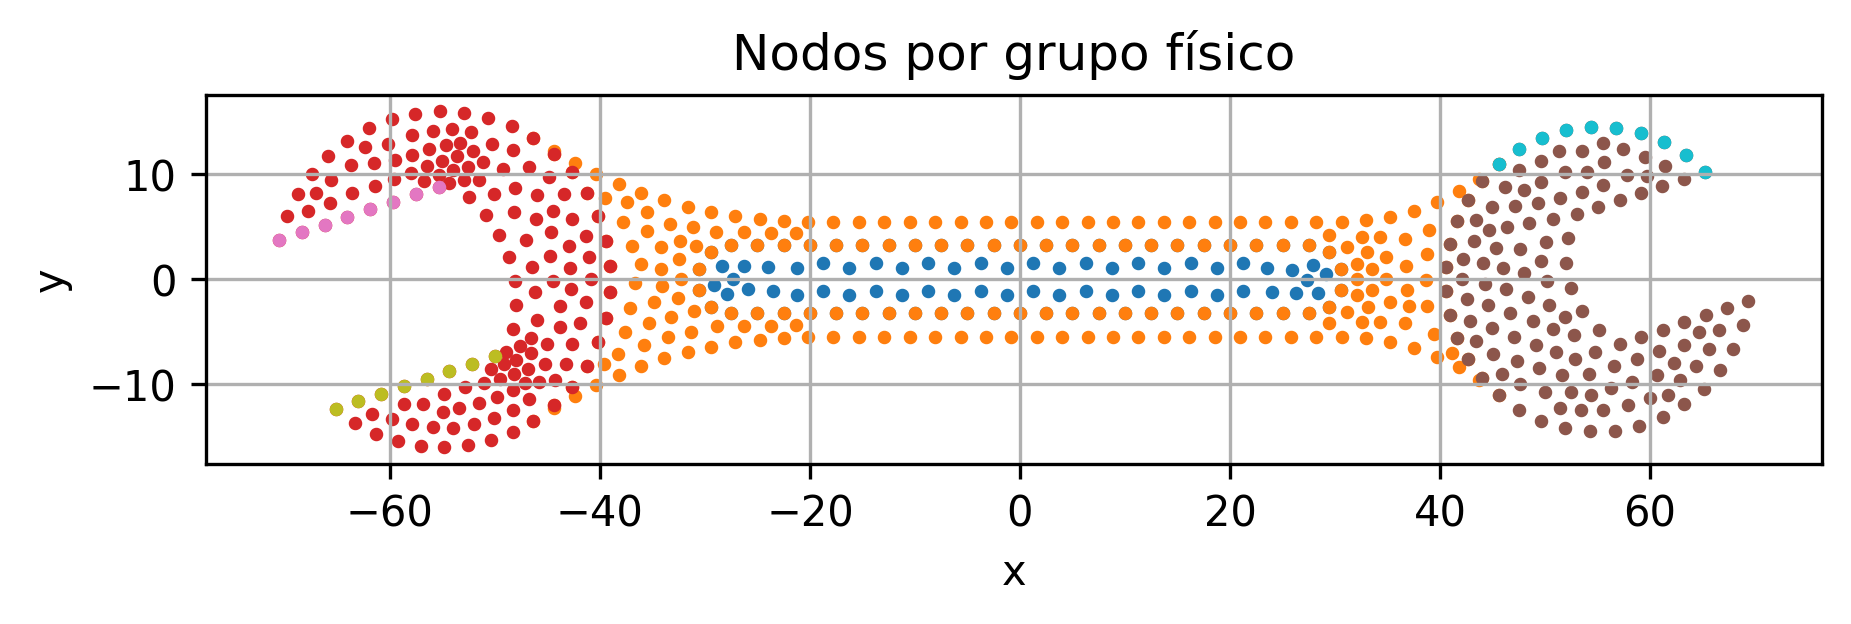
\includegraphics[width=0.8\textwidth]{GRAFICOS/Case a_nodes_por_grupo.png}
  \caption{Caption}
  \label{fig:wrench}
\end{figure}

\begin{figure}[H]
  \centering
  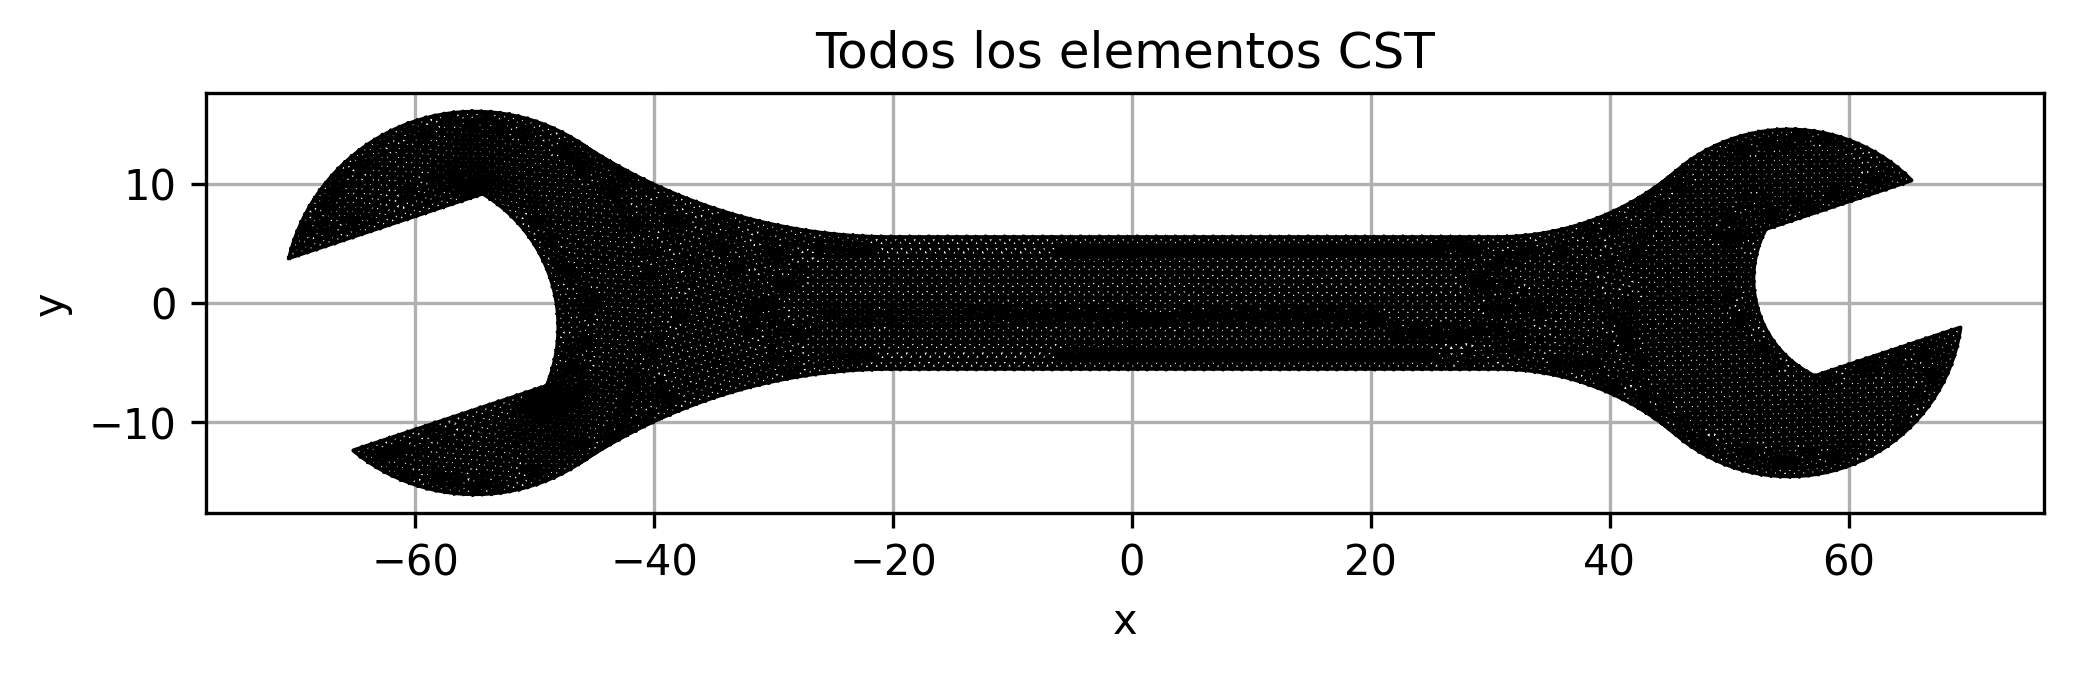
\includegraphics[width=0.8\textwidth]{GRAFICOS/Case a_elementos.png}
  \caption{Caption}
  \label{fig:deformed_shape}
\end{figure}

\begin{figure}[H]
  \centering
  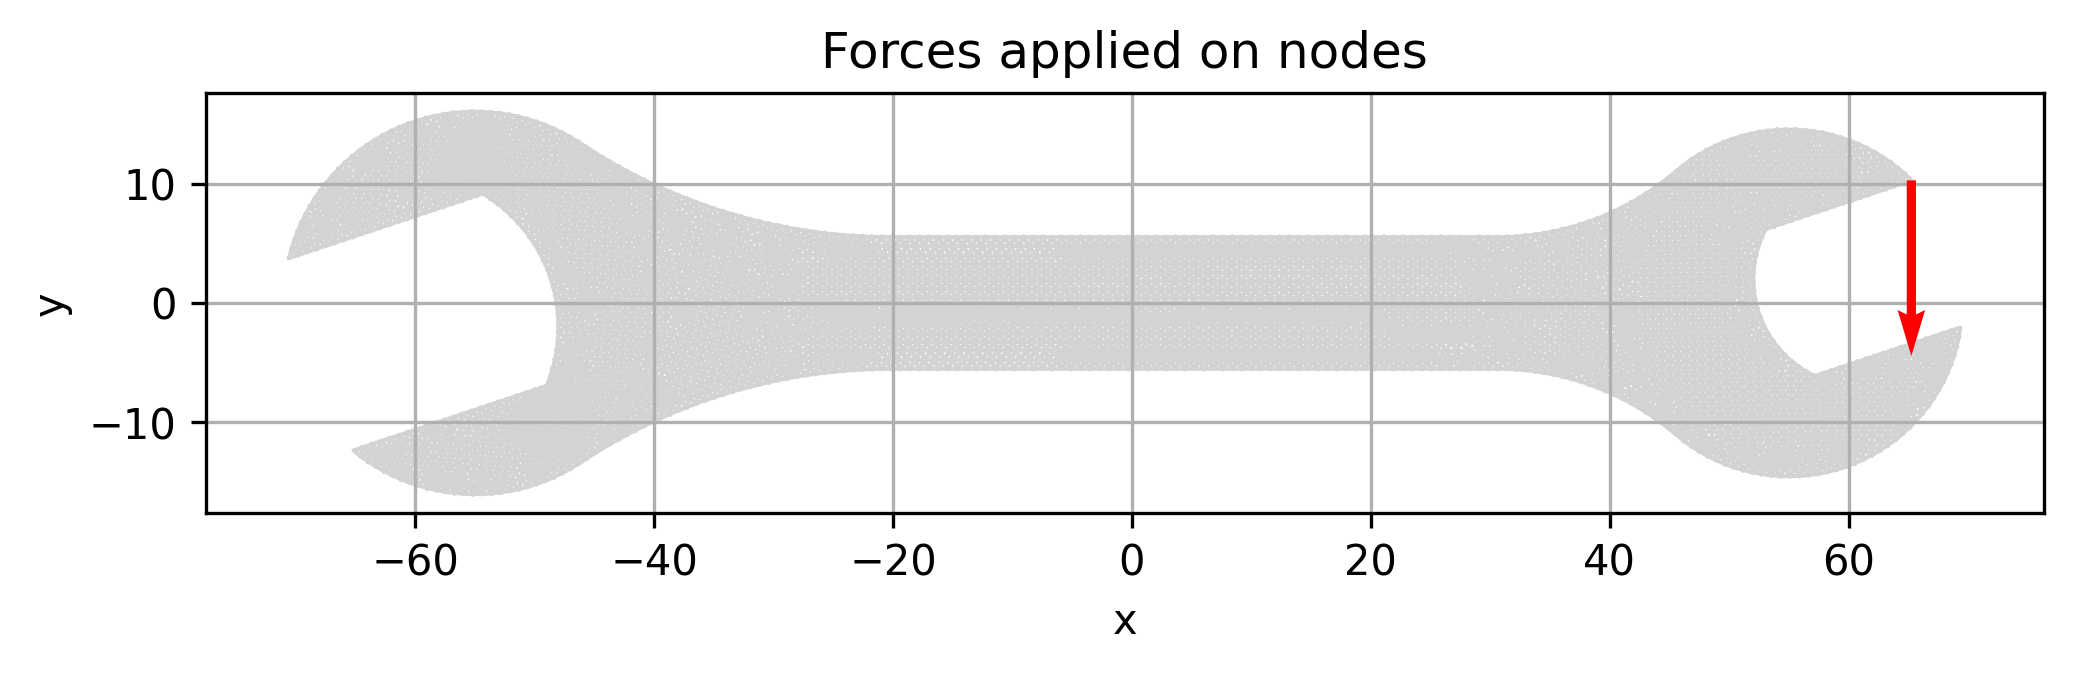
\includegraphics[width=0.8\textwidth]{GRAFICOS/Case a_fuerzas.png}
  \caption{Caption}
  \label{fig:strain}
\end{figure}

\begin{figure}[H]
  \centering
  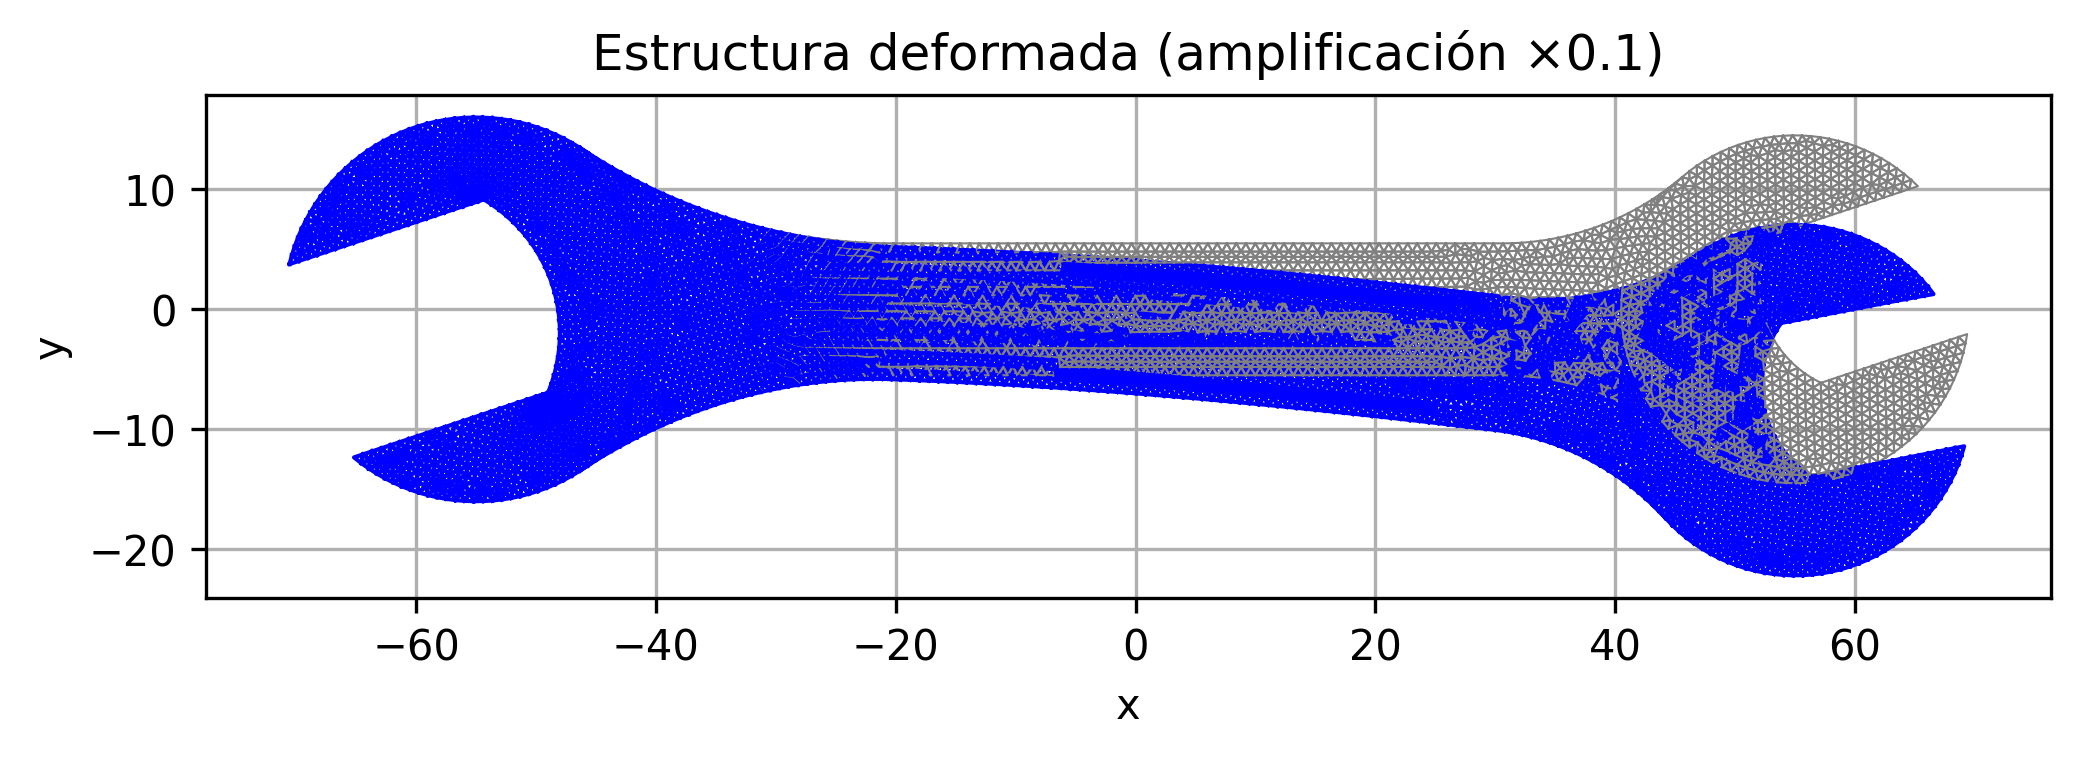
\includegraphics[width=0.8\textwidth]{GRAFICOS/Case a_deformada.png}
  \caption{Caption}
  \label{fig:stress}
\end{figure}

\begin{figure}[H]
  \centering
  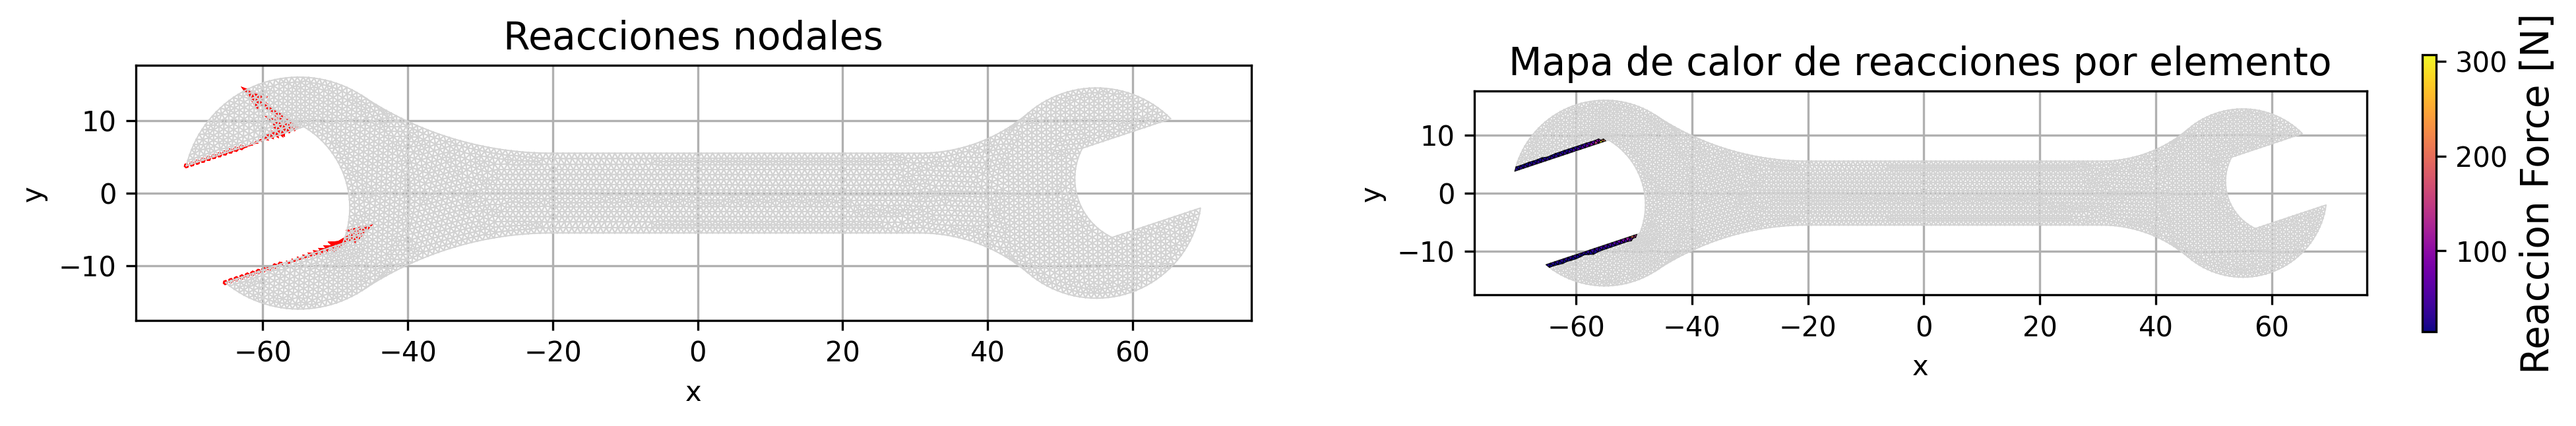
\includegraphics[width=1\textwidth]{GRAFICOS/Case a_deformada_reacciones.png}
  \caption{Caption}
  \label{fig:principal}
\end{figure}

\begin{figure}[H]
  \centering
  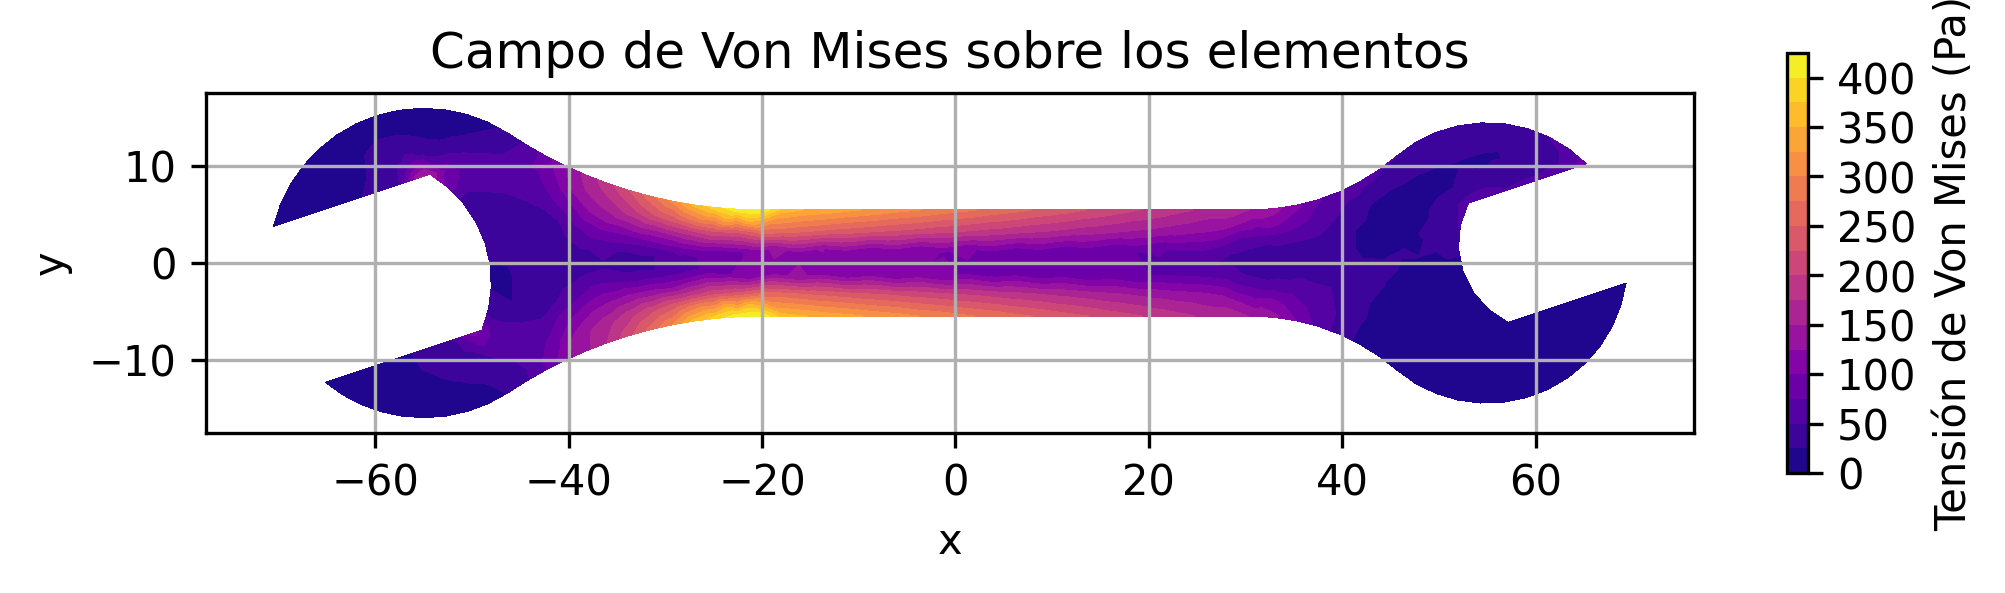
\includegraphics[width=0.8\textwidth]{GRAFICOS/Case a_von_mises.png}
  \caption{Caption}
  \label{fig:principal}
\end{figure}

\begin{figure}[H]
  \centering
  \begin{subfigure}[t]{0.49\textwidth}
    \centering
    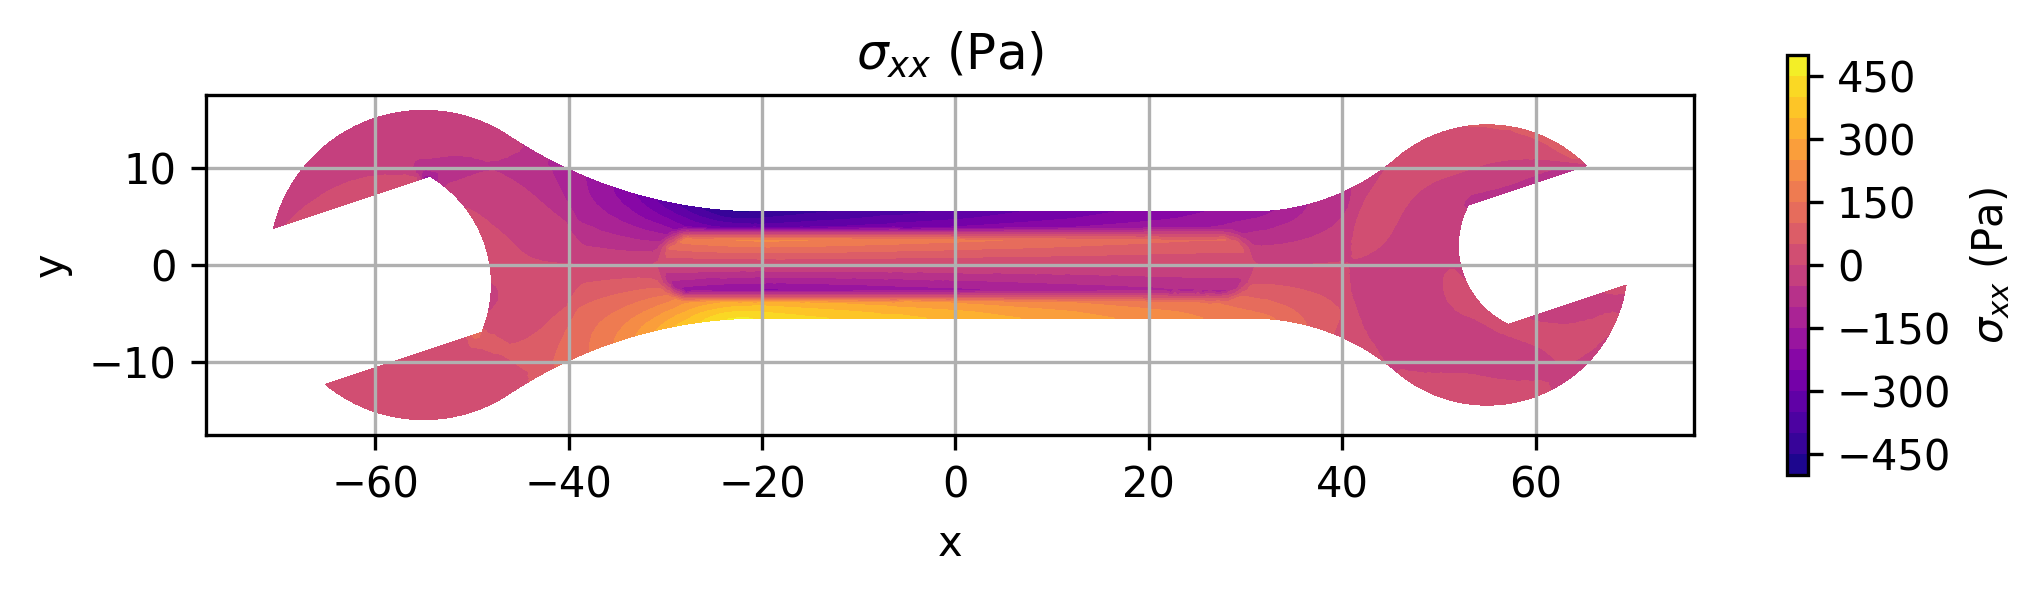
\includegraphics[width=\textwidth]{GRAFICOS/Case a - sigma_xx.png}
    \caption{Caption}
    \label{fig:deformada_reacciones}
  \end{subfigure}
  \hfill
  \begin{subfigure}[t]{0.49\textwidth}
    \centering
    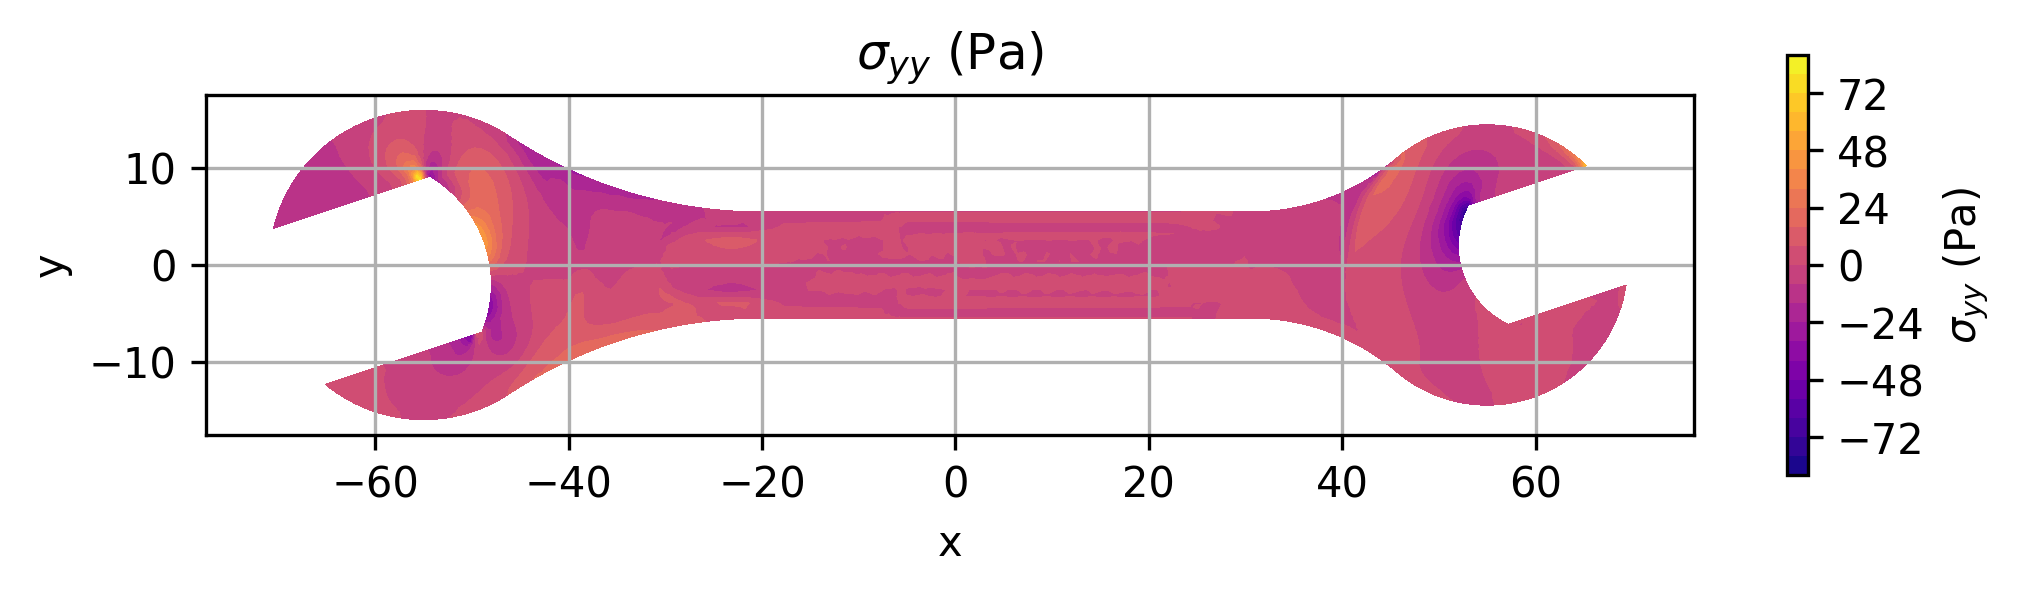
\includegraphics[width=\textwidth]{GRAFICOS/Case a - sigma_yy.png}
    \caption{Caption}
    \label{fig:von_mises}
  \end{subfigure}
  \caption{Caption}
  \label{fig:analisis_estructural}
\end{figure}

\begin{figure}[H]
  \centering
  \begin{subfigure}[t]{0.49\textwidth}
    \centering
    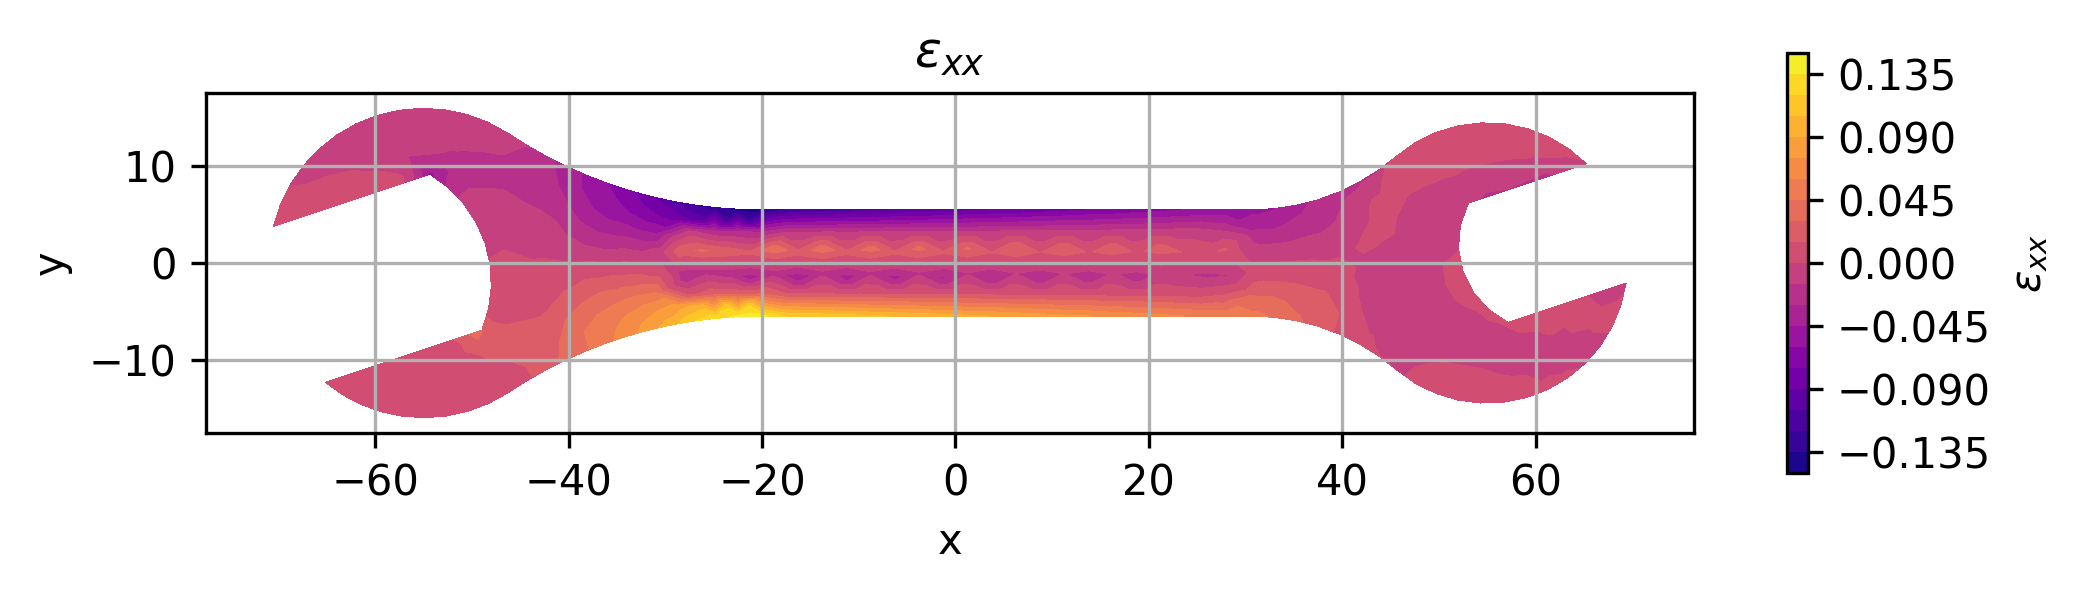
\includegraphics[width=\textwidth]{GRAFICOS/Case a - epsilon_xx.png}
    \caption{Caption}
    \label{fig:deformada_reacciones}
  \end{subfigure}
  \hfill
  \begin{subfigure}[t]{0.49\textwidth}
    \centering
    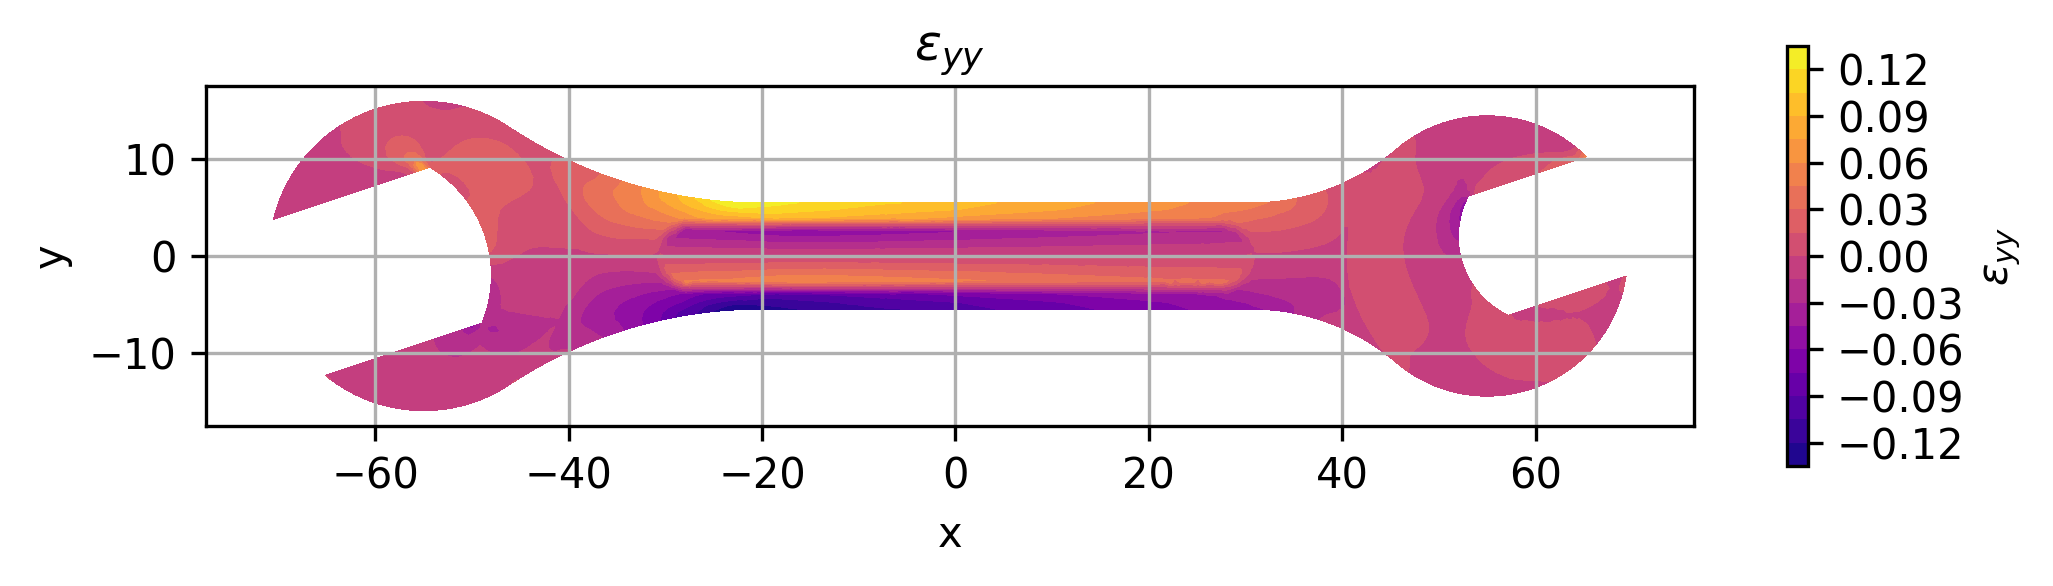
\includegraphics[width=\textwidth]{GRAFICOS/Case a - epsilon_yy.png}
    \caption{Caption}
    \label{fig:von_mises}
  \end{subfigure}
  \caption{Caption}
  \label{fig:analisis_estructural}
\end{figure}

\begin{figure}[H]
  \centering
  \begin{subfigure}[t]{0.49\textwidth}
    \centering
    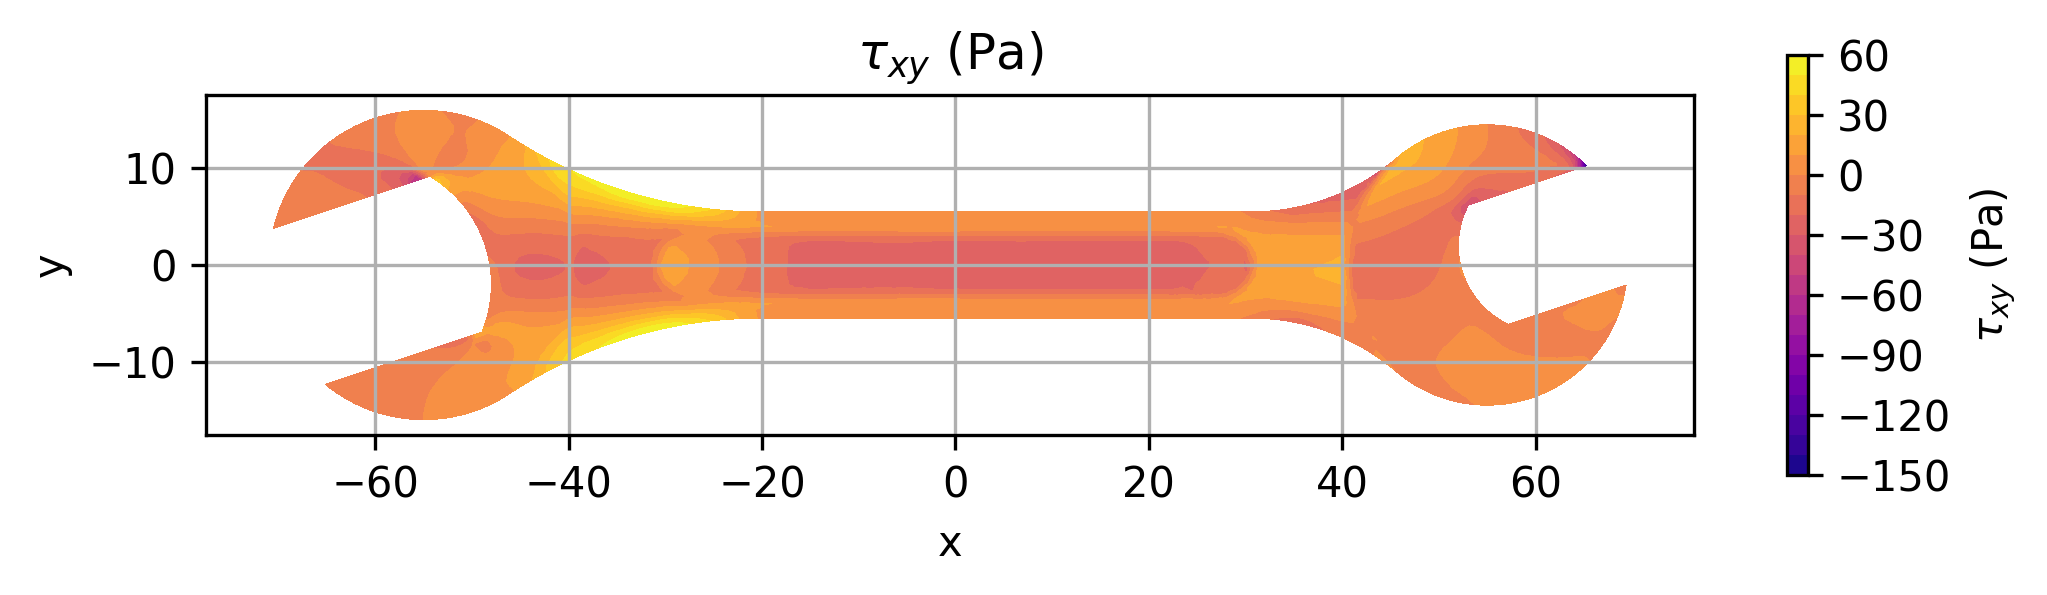
\includegraphics[width=\textwidth]{GRAFICOS/Case a - tau_xy.png}
    \caption{Caption}
    \label{fig:deformada_reacciones}
  \end{subfigure}
  \hfill
  \begin{subfigure}[t]{0.49\textwidth}
    \centering
    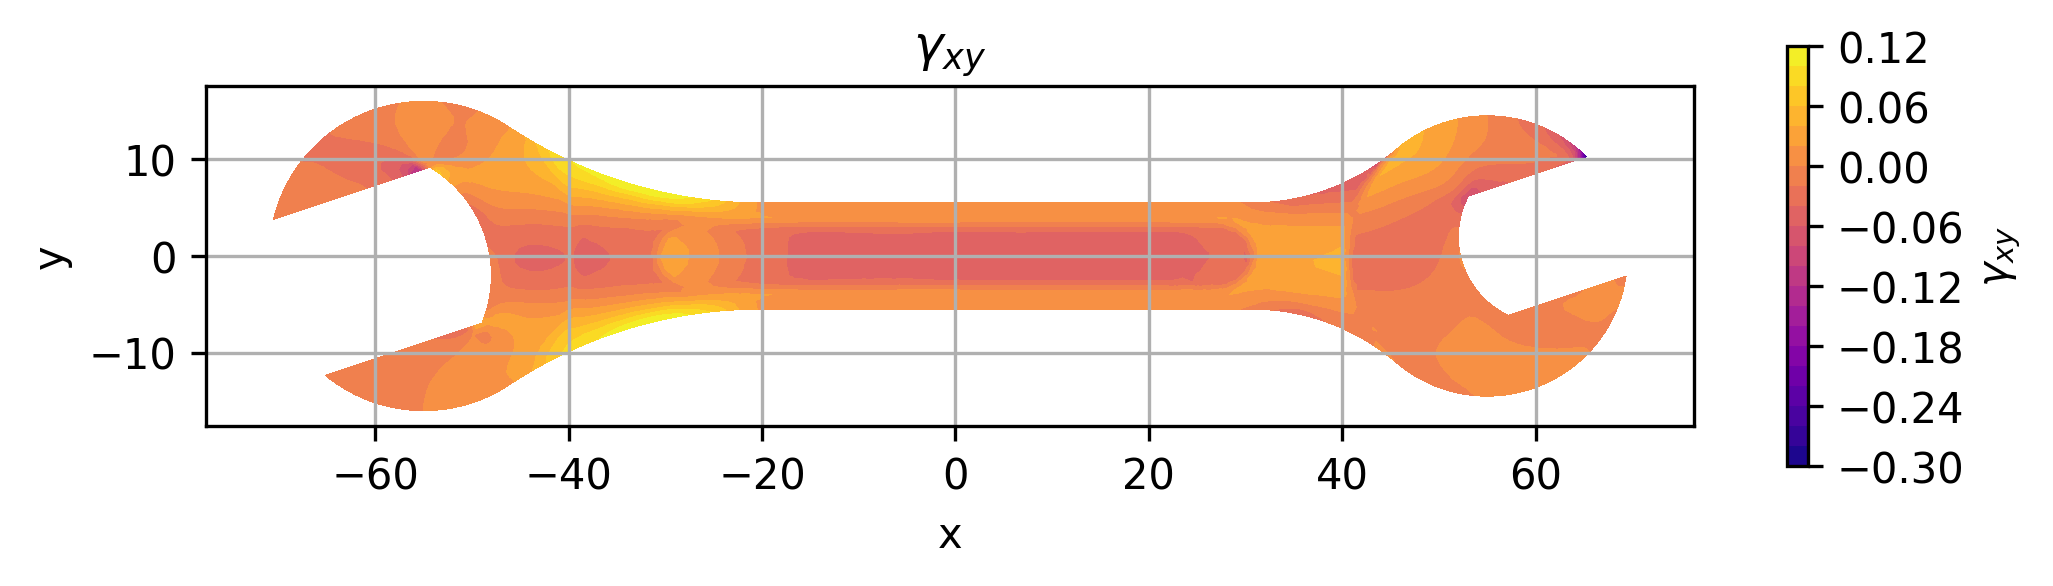
\includegraphics[width=\textwidth]{GRAFICOS/Case a - gamma_xy.png}
    \caption{Caption}
    \label{fig:von_mises}
  \end{subfigure}
  \caption{Caption}
  \label{fig:analisis_estructural}
\end{figure}

\begin{figure}[H]
  \centering
  \begin{subfigure}[t]{0.49\textwidth}
    \centering
    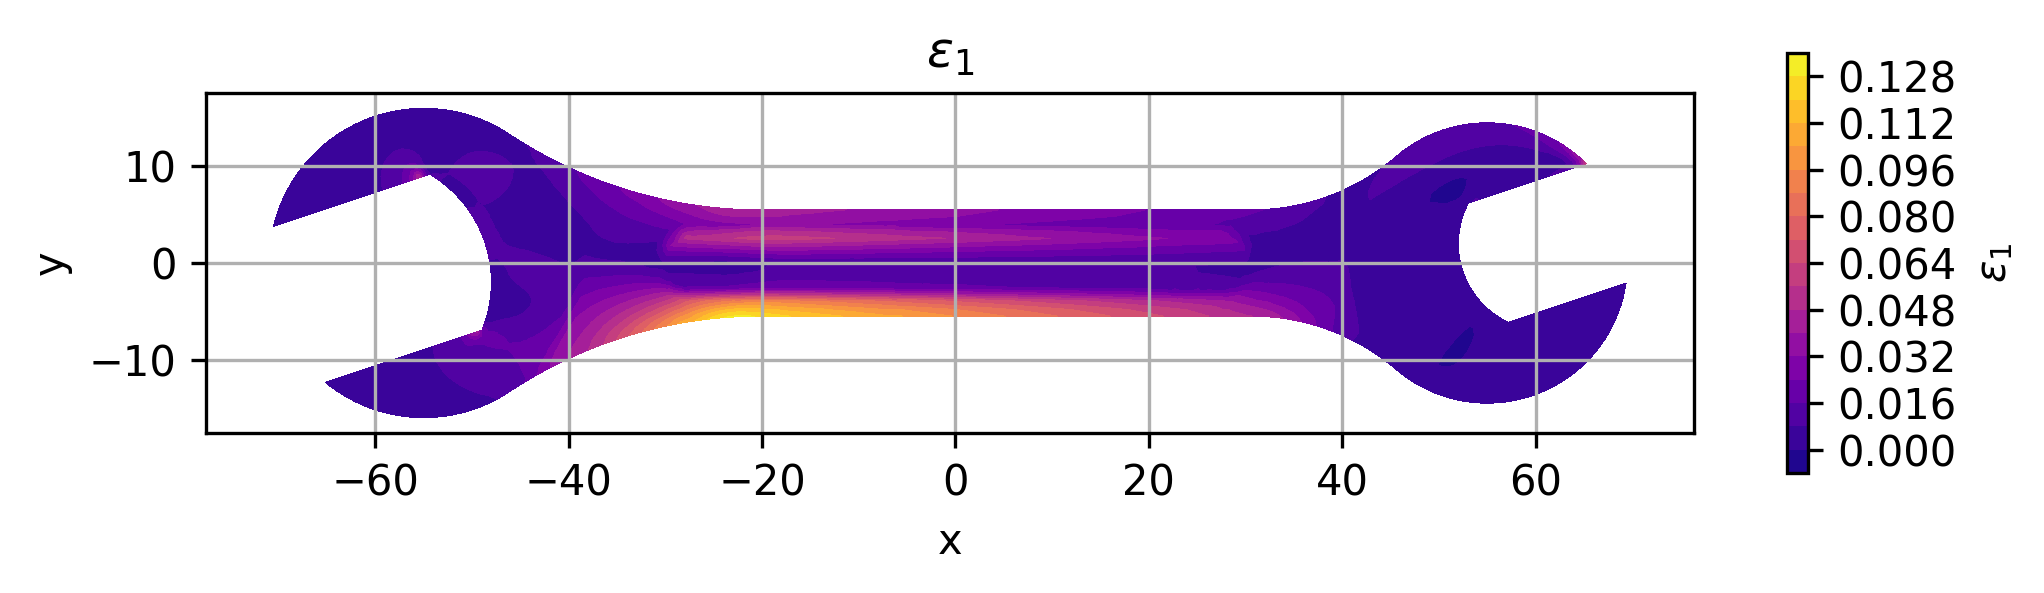
\includegraphics[width=\textwidth]{GRAFICOS/Case a - epsilon_1.png}
    \caption{Caption}
    \label{fig:deformada_reacciones}
  \end{subfigure}
  \hfill
  \begin{subfigure}[t]{0.49\textwidth}
    \centering
    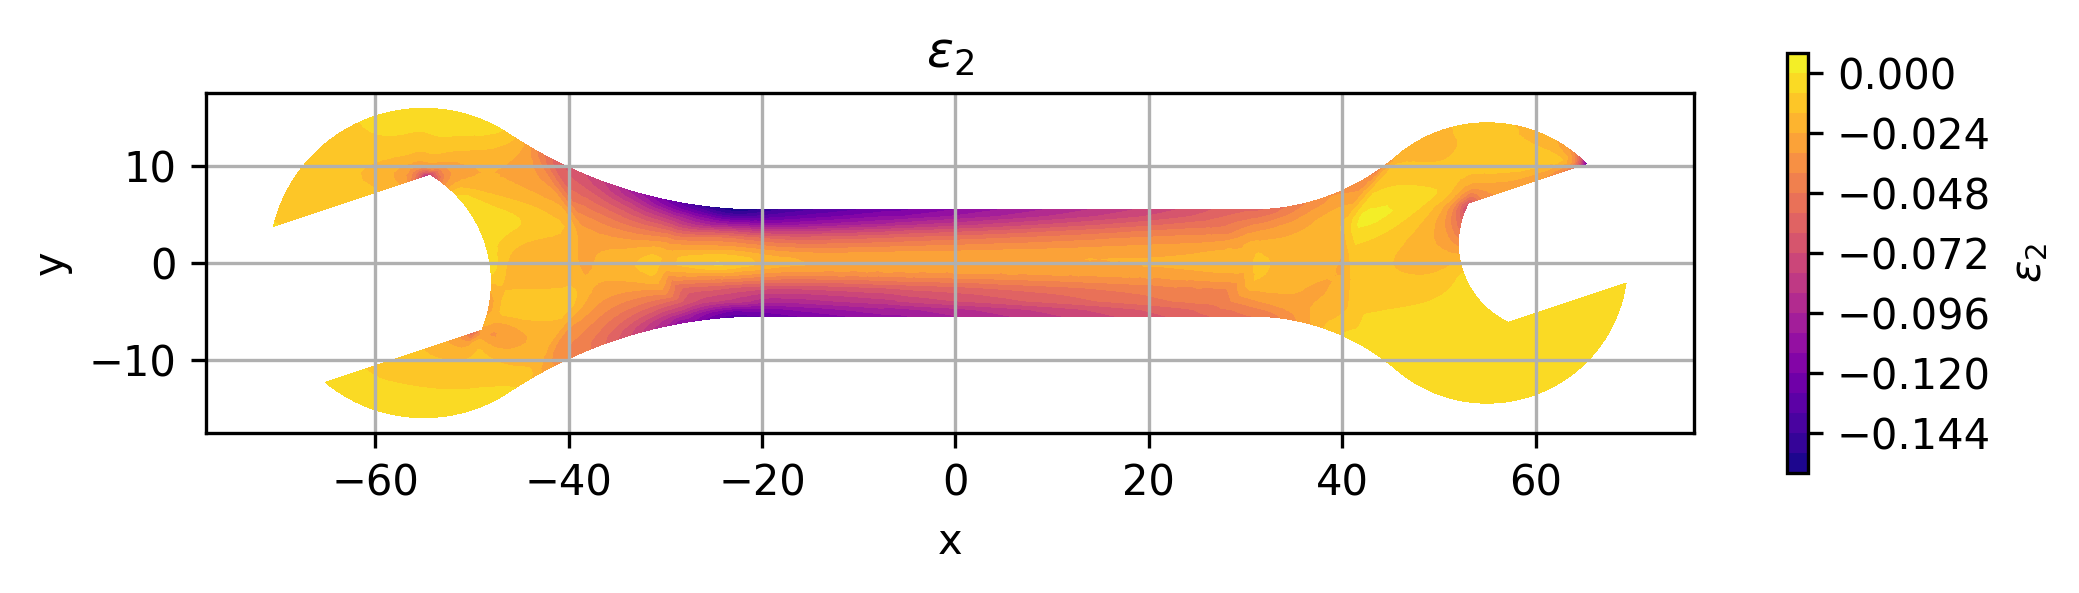
\includegraphics[width=\textwidth]{GRAFICOS/Case a - epsilon_2.png}
    \caption{Caption}
    \label{fig:von_mises}
  \end{subfigure}
  \caption{Caption}
  \label{fig:analisis_estructural}
\end{figure}

\begin{figure}[H]
  \centering
  \begin{subfigure}[t]{0.49\textwidth}
    \centering
    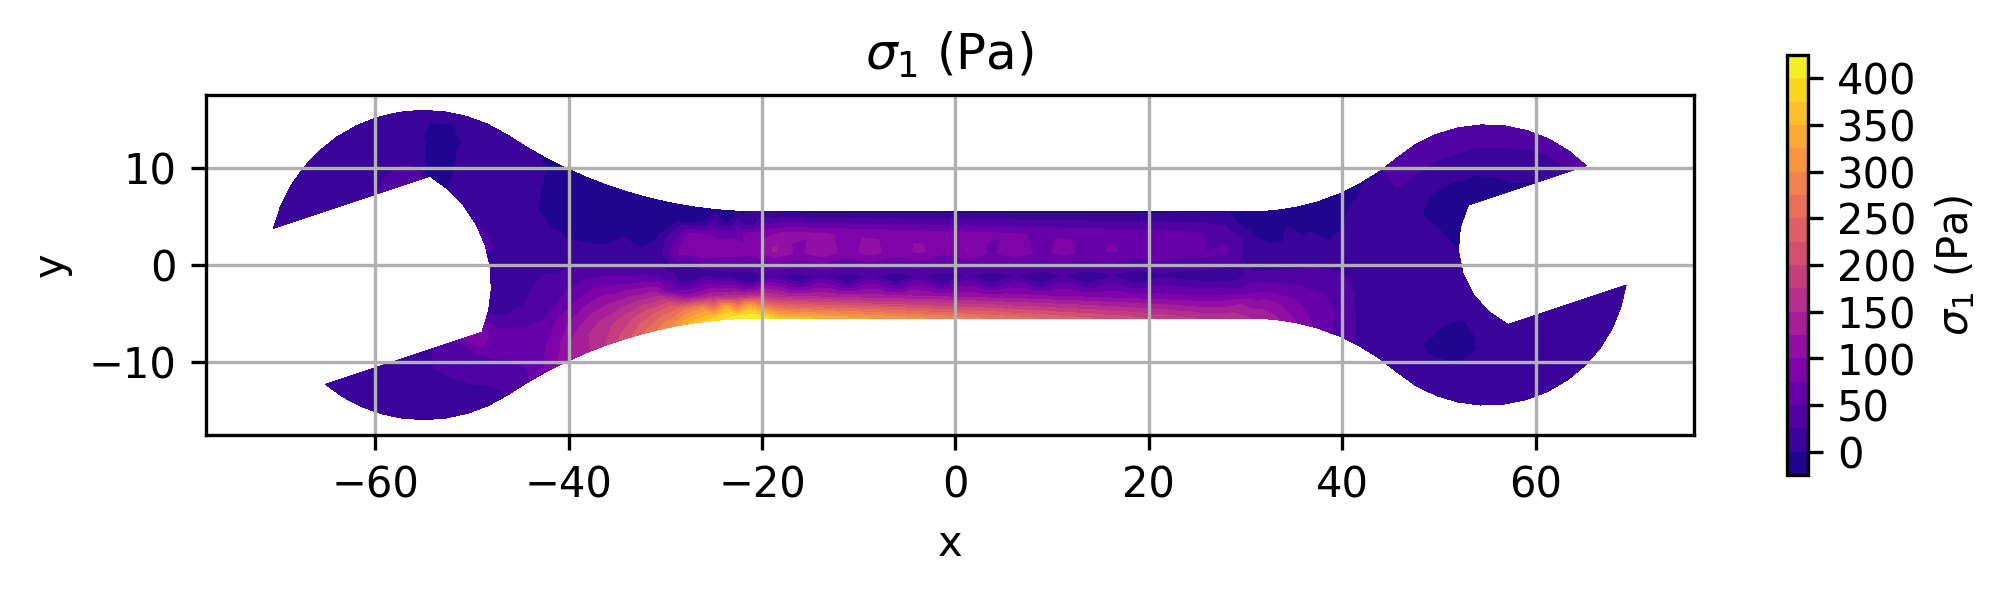
\includegraphics[width=\textwidth]{GRAFICOS/Case a - sigma_1.png}
    \caption{Caption}
    \label{fig:deformada_reacciones}
  \end{subfigure}
  \hfill
  \begin{subfigure}[t]{0.49\textwidth}
    \centering
    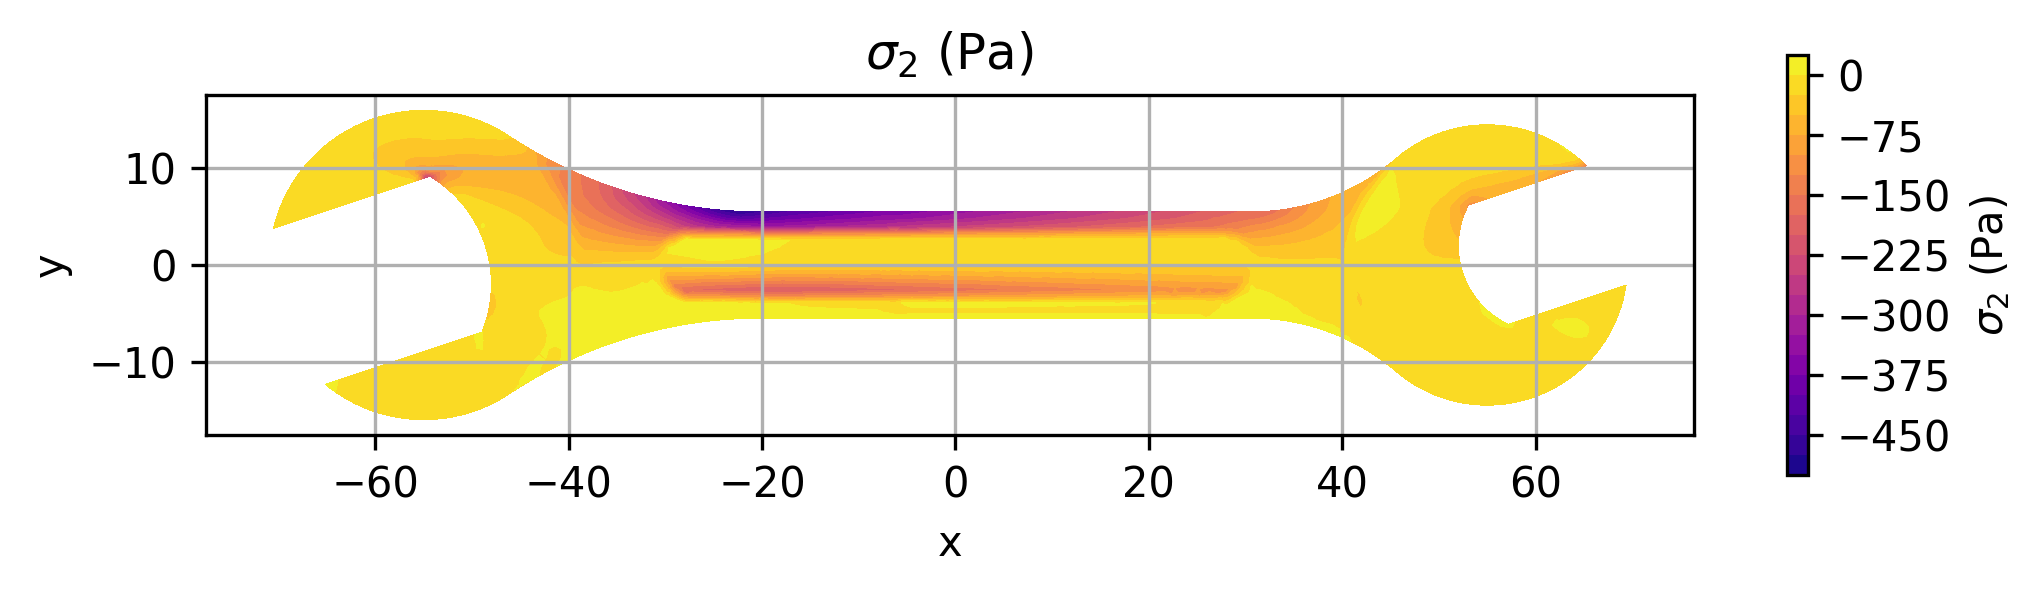
\includegraphics[width=\textwidth]{GRAFICOS/Case a - sigma_2.png}
    \caption{Caption}
    \label{fig:von_mises}
  \end{subfigure}
  \caption{Caption}
  \label{fig:analisis_estructural}
\end{figure}



\section{B case}

\begin{figure}[H]
  \centering
  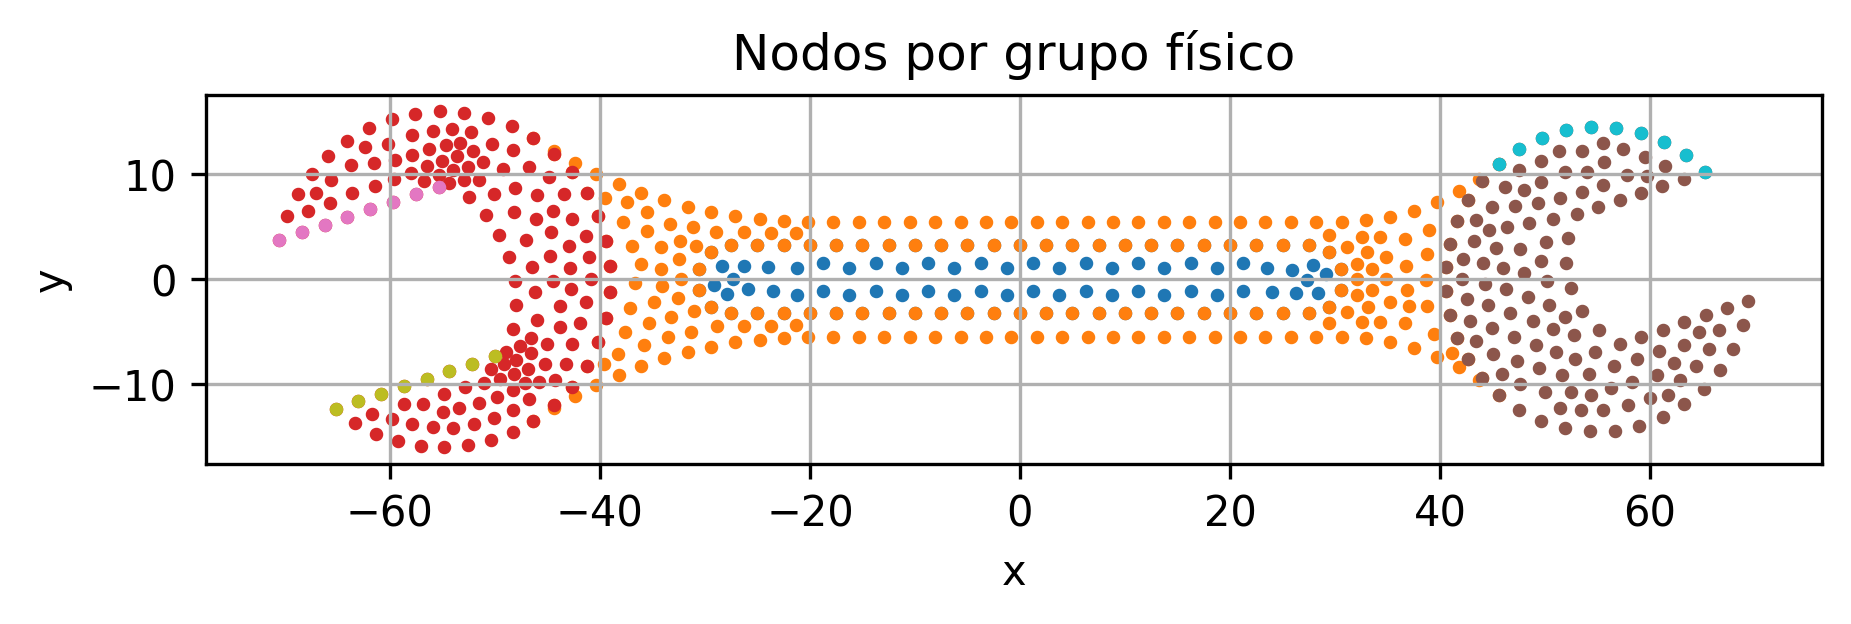
\includegraphics[width=0.8\textwidth]{GRAFICOS/Case b_nodes_por_grupo.png}
  \caption{Caption}
  \label{fig:wrench}
\end{figure}

\begin{figure}[H]
  \centering
  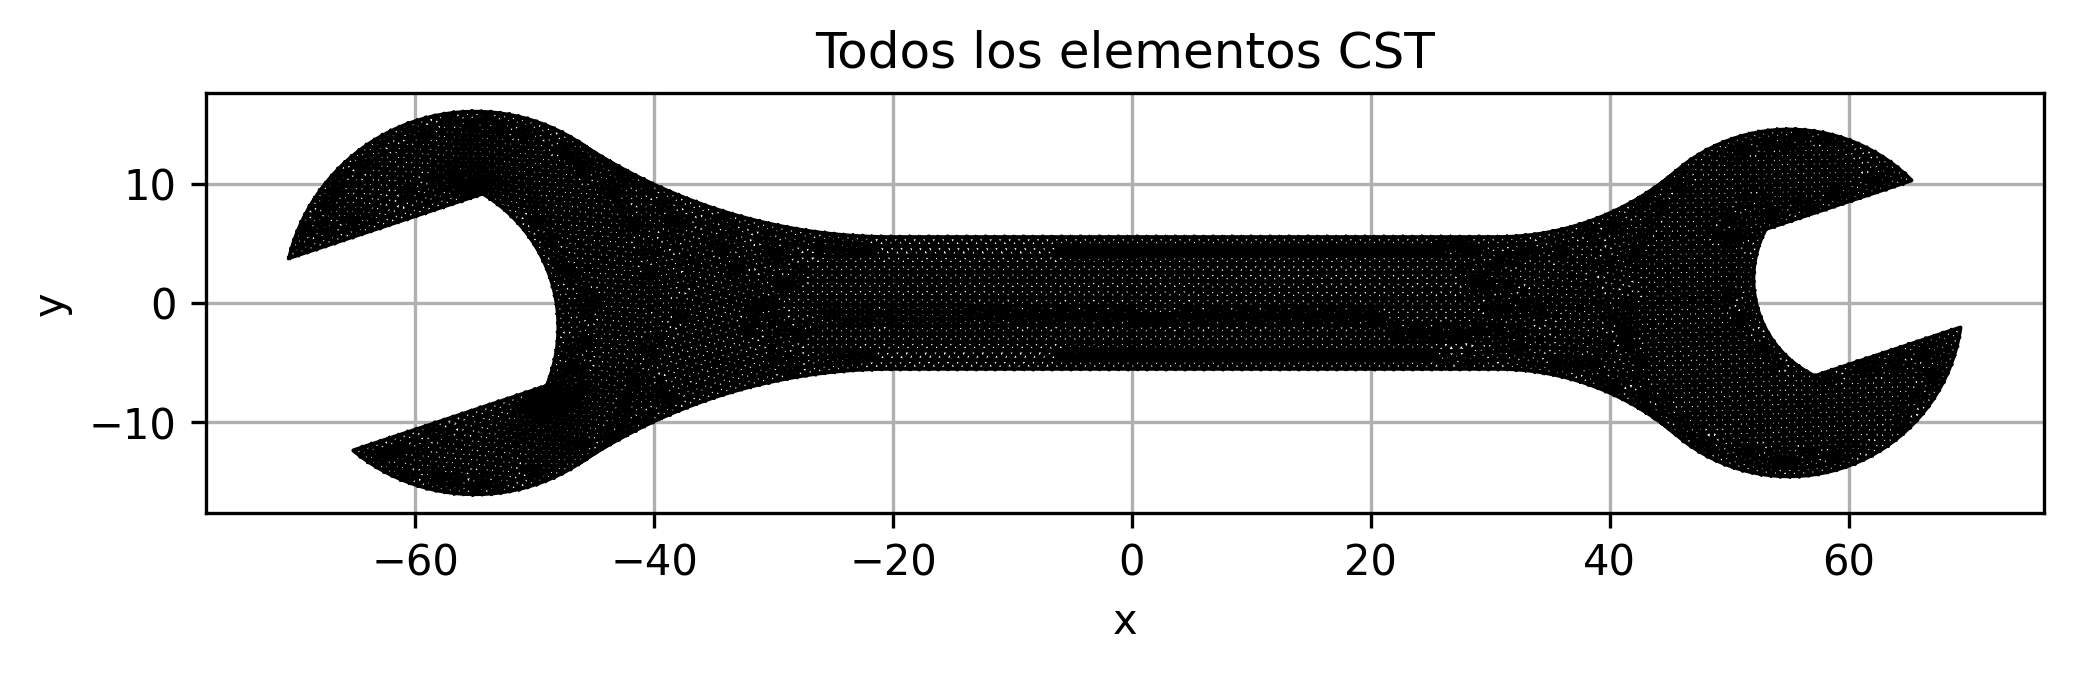
\includegraphics[width=0.8\textwidth]{GRAFICOS/Case b_elementos.png}
  \caption{Caption}
  \label{fig:deformed_shape}
\end{figure}

\begin{figure}[H]
  \centering
  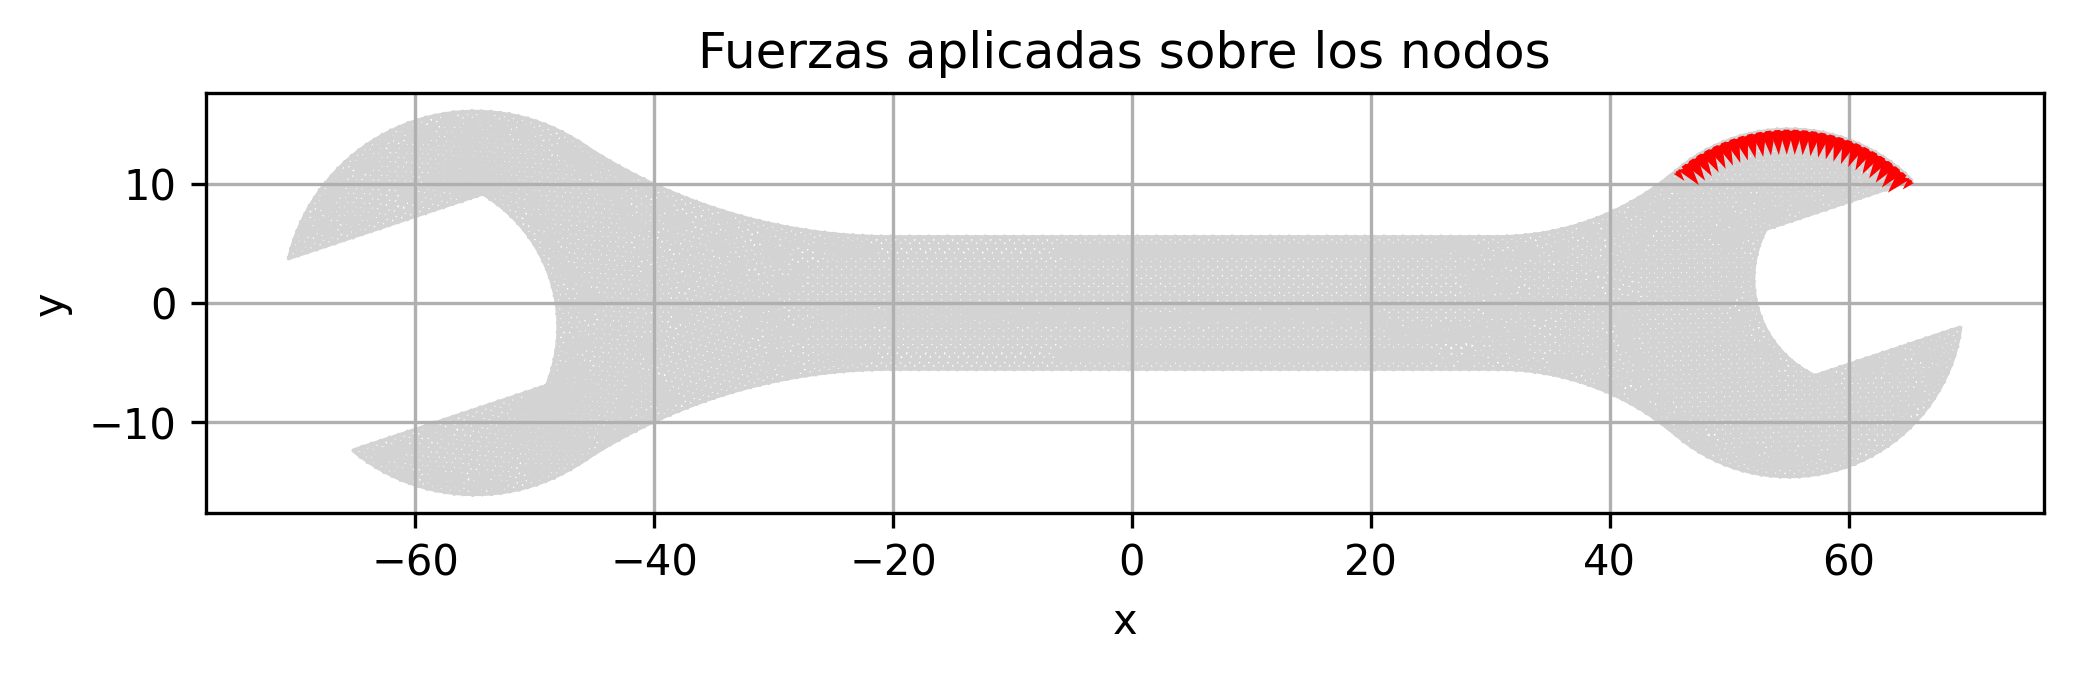
\includegraphics[width=0.8\textwidth]{GRAFICOS/Case b_fuerzas.png}
  \caption{Caption}
  \label{fig:strain}
\end{figure}

\begin{figure}[H]
  \centering
  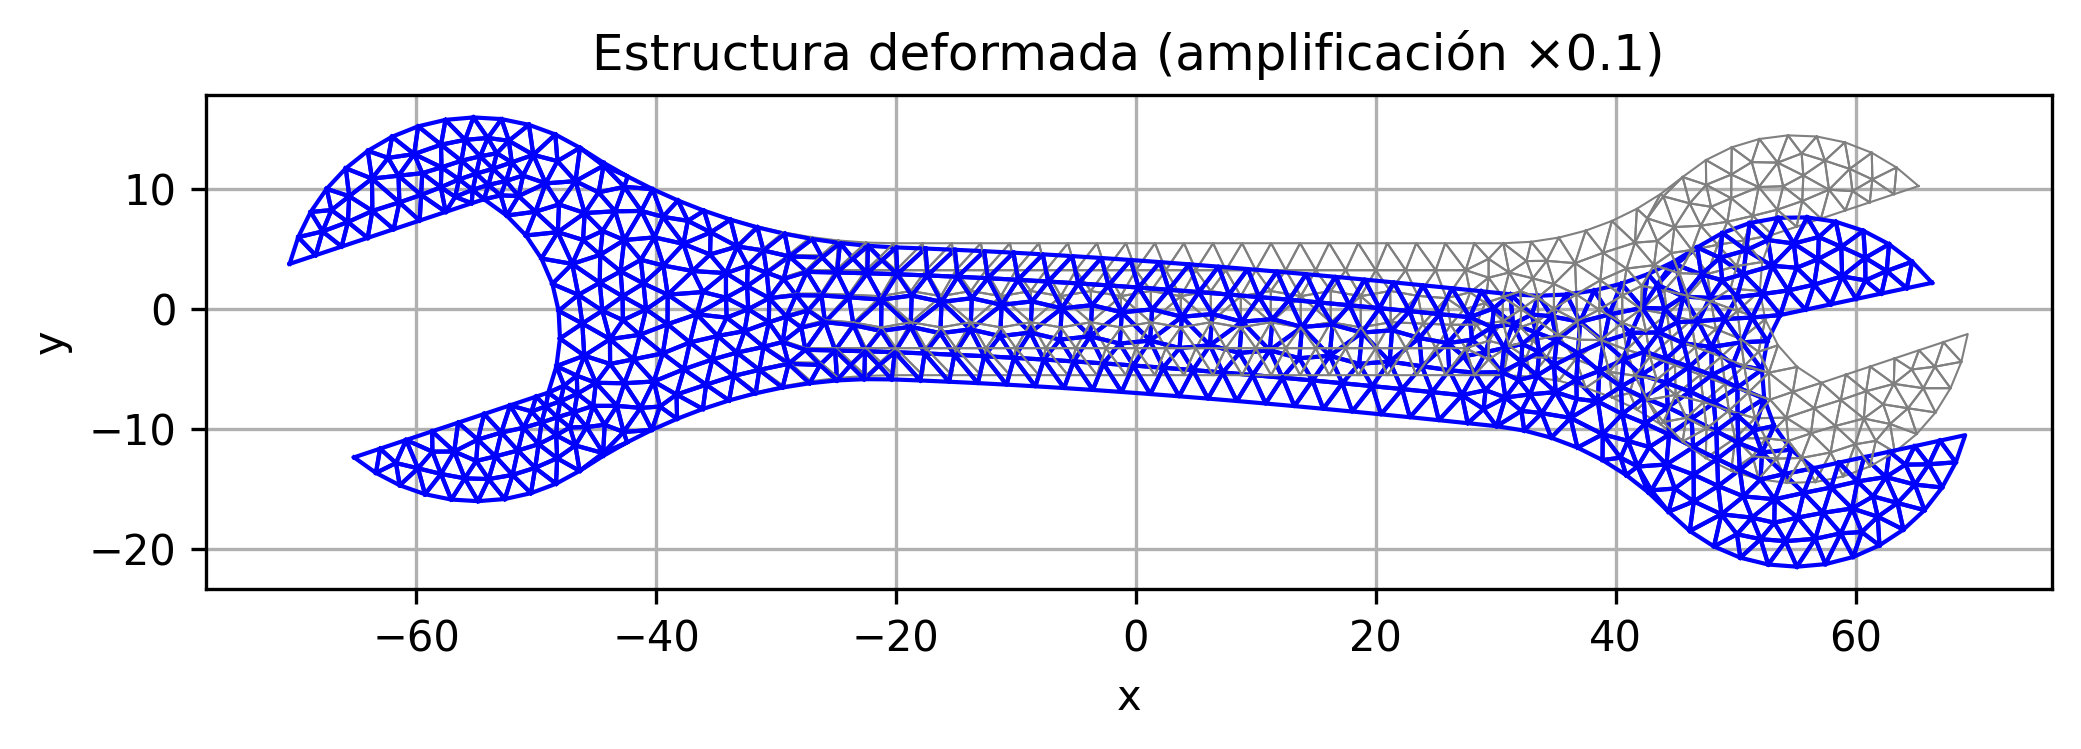
\includegraphics[width=0.8\textwidth]{GRAFICOS/Case b_deformada.png}
  \caption{Caption}
  \label{fig:stress}
\end{figure}

\begin{figure}[H]
  \centering
  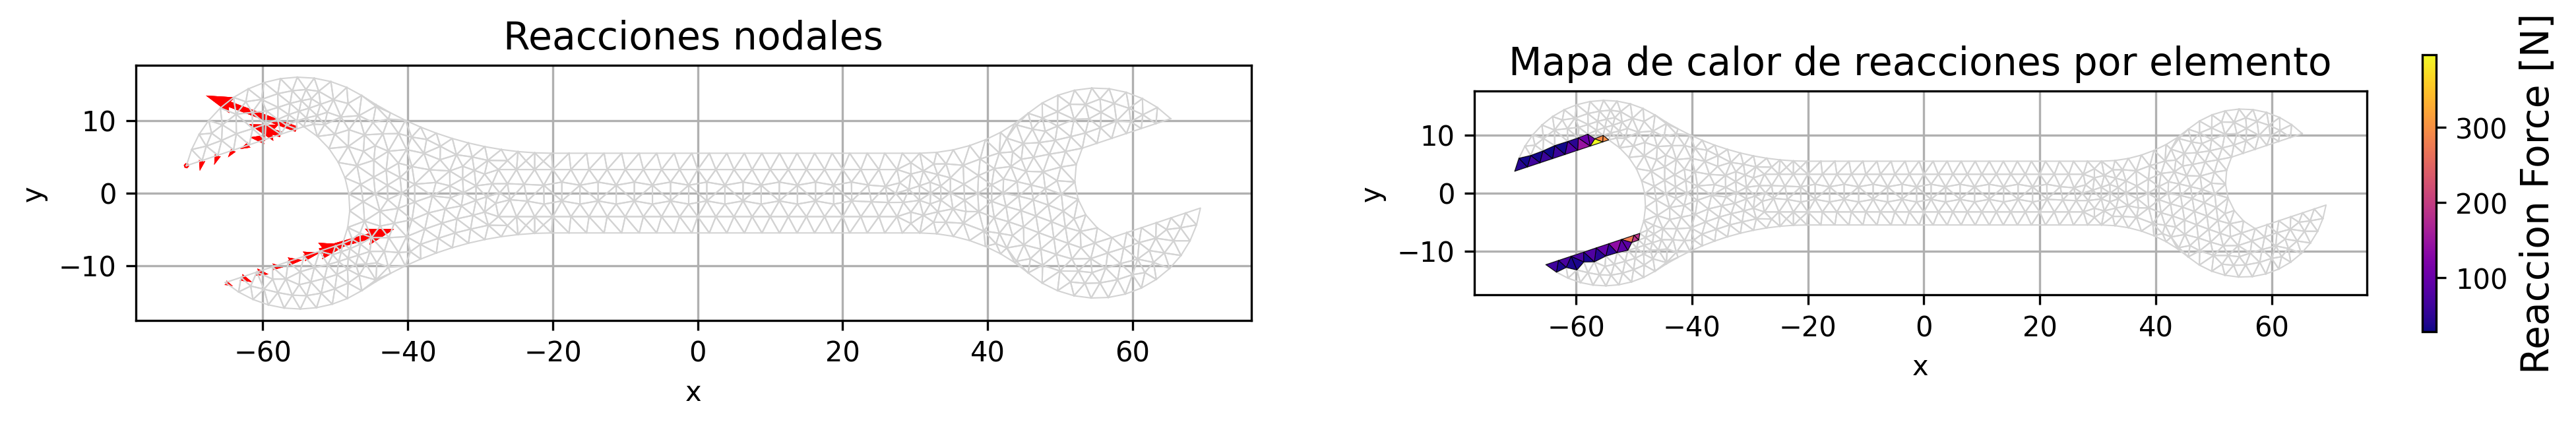
\includegraphics[width=1\textwidth]{GRAFICOS/Case b_deformada_reacciones.png}
  \caption{Caption}
  \label{fig:principal}
\end{figure}

\begin{figure}[H]
  \centering
  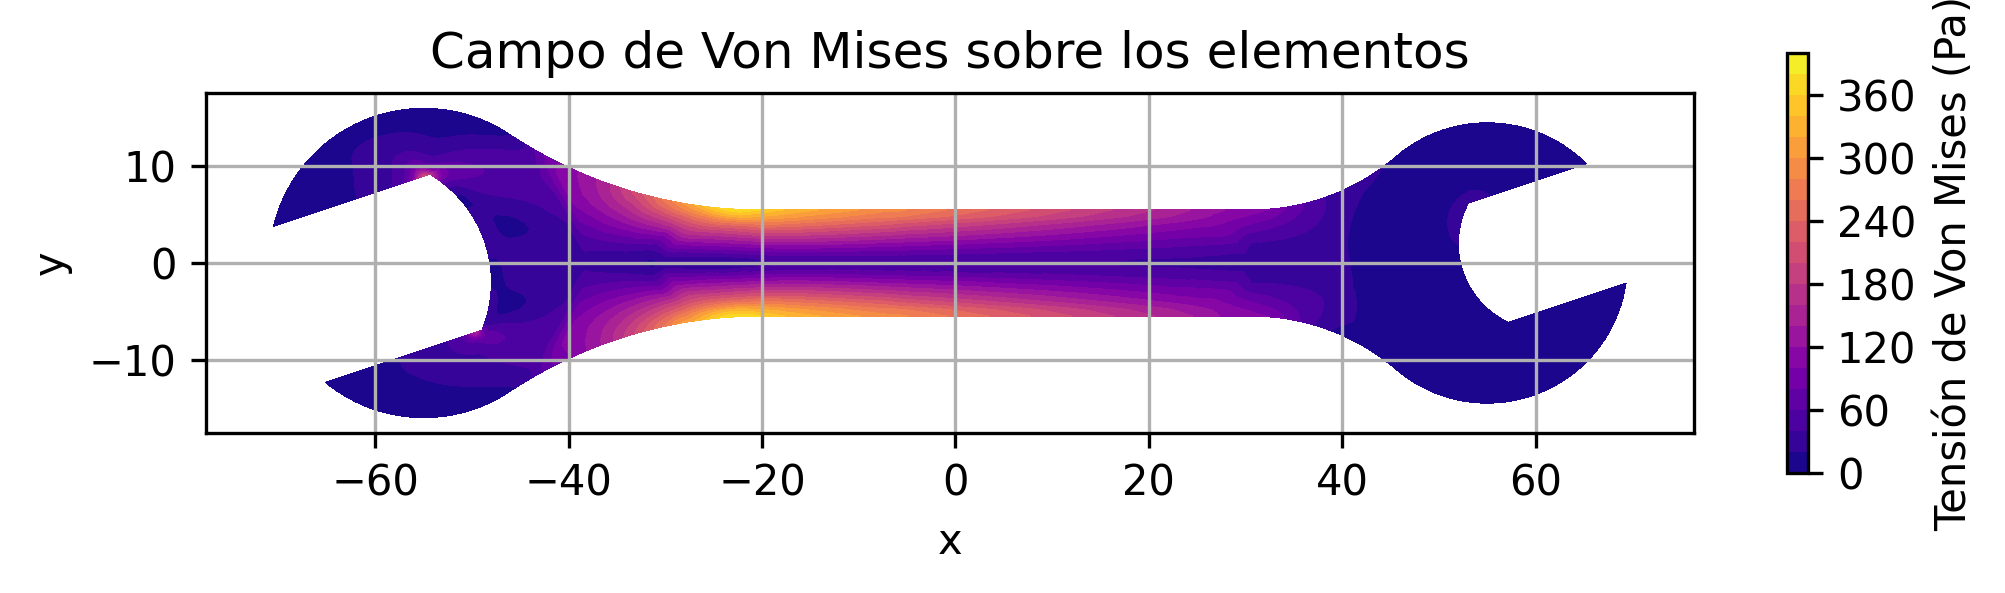
\includegraphics[width=0.8\textwidth]{GRAFICOS/Case b_von_mises.png}
  \caption{Caption}
  \label{fig:principal}
\end{figure}

\begin{figure}[H]
  \centering
  \begin{subfigure}[t]{0.49\textwidth}
    \centering
    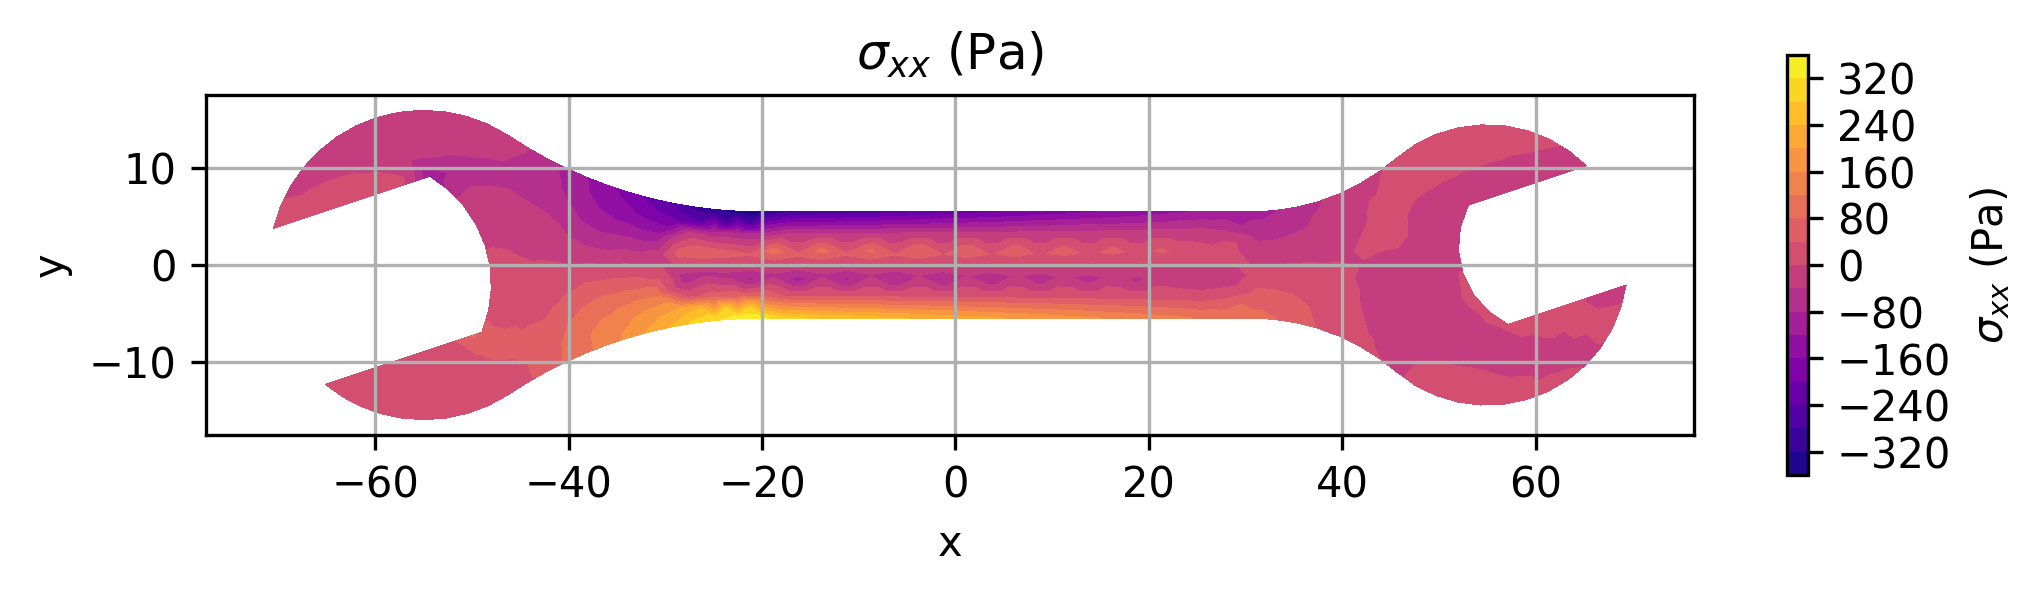
\includegraphics[width=\textwidth]{GRAFICOS/Case b - sigma_xx.png}
    \caption{Caption}
    \label{fig:deformada_reacciones}
  \end{subfigure}
  \hfill
  \begin{subfigure}[t]{0.49\textwidth}
    \centering
    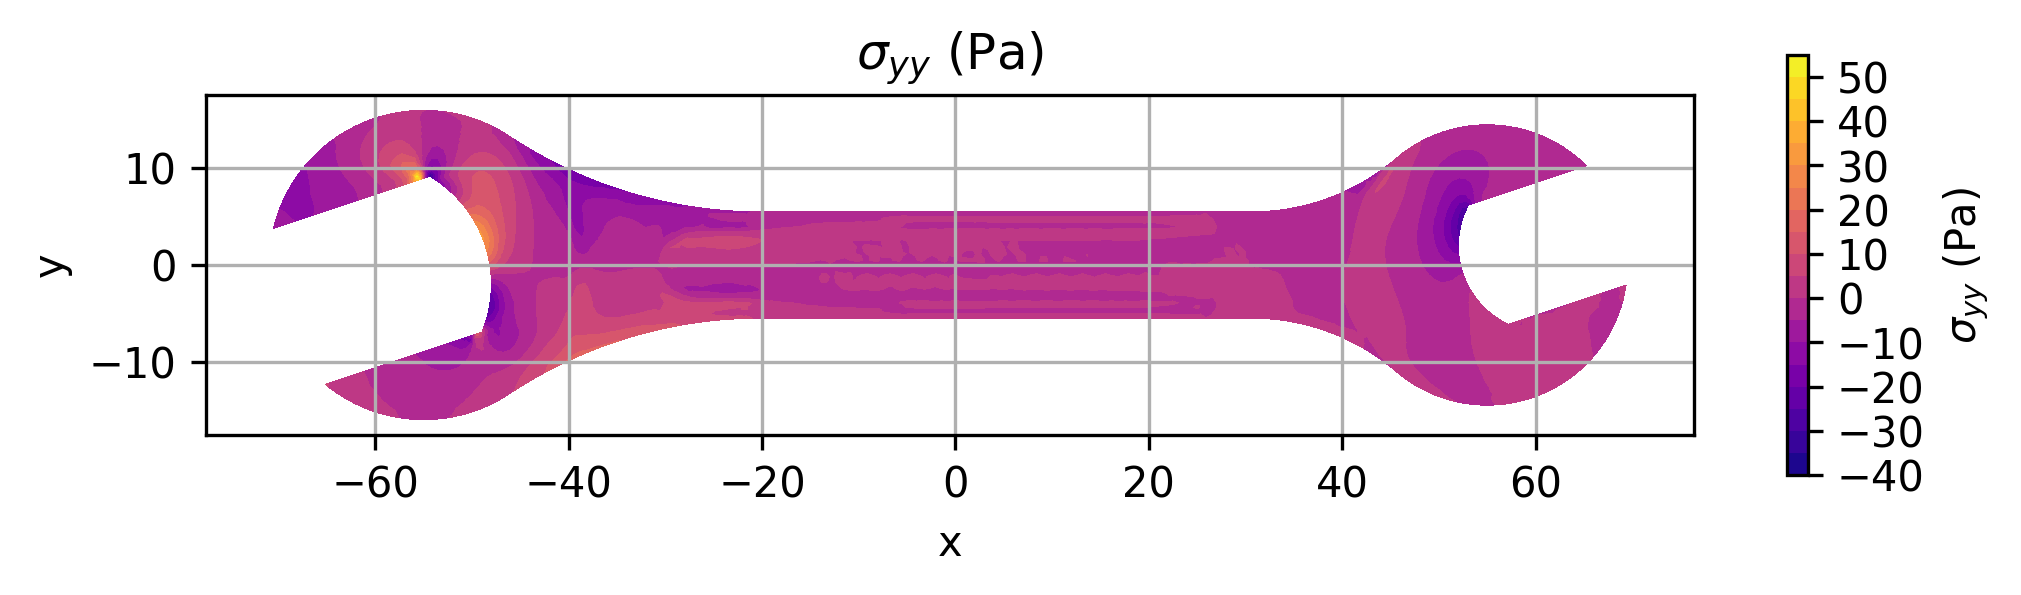
\includegraphics[width=\textwidth]{GRAFICOS/Case b - sigma_yy.png}
    \caption{Caption}
    \label{fig:von_mises}
  \end{subfigure}
  \caption{Caption}
  \label{fig:analisis_estructural}
\end{figure}

\begin{figure}[H]
  \centering
  \begin{subfigure}[t]{0.49\textwidth}
    \centering
    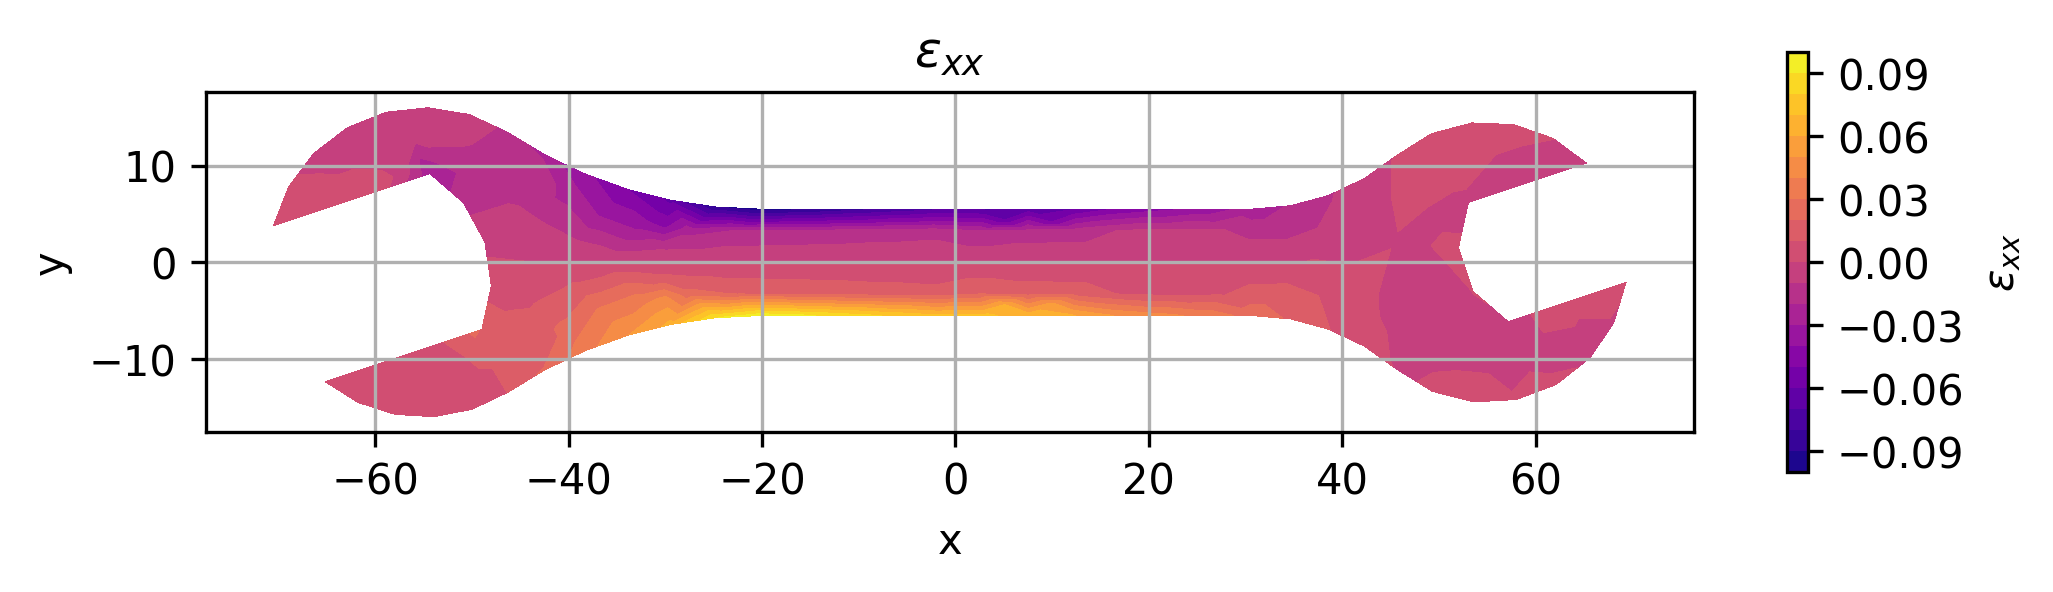
\includegraphics[width=\textwidth]{GRAFICOS/Case b - epsilon_xx.png}
    \caption{Caption}
    \label{fig:deformada_reacciones}
  \end{subfigure}
  \hfill
  \begin{subfigure}[t]{0.49\textwidth}
    \centering
    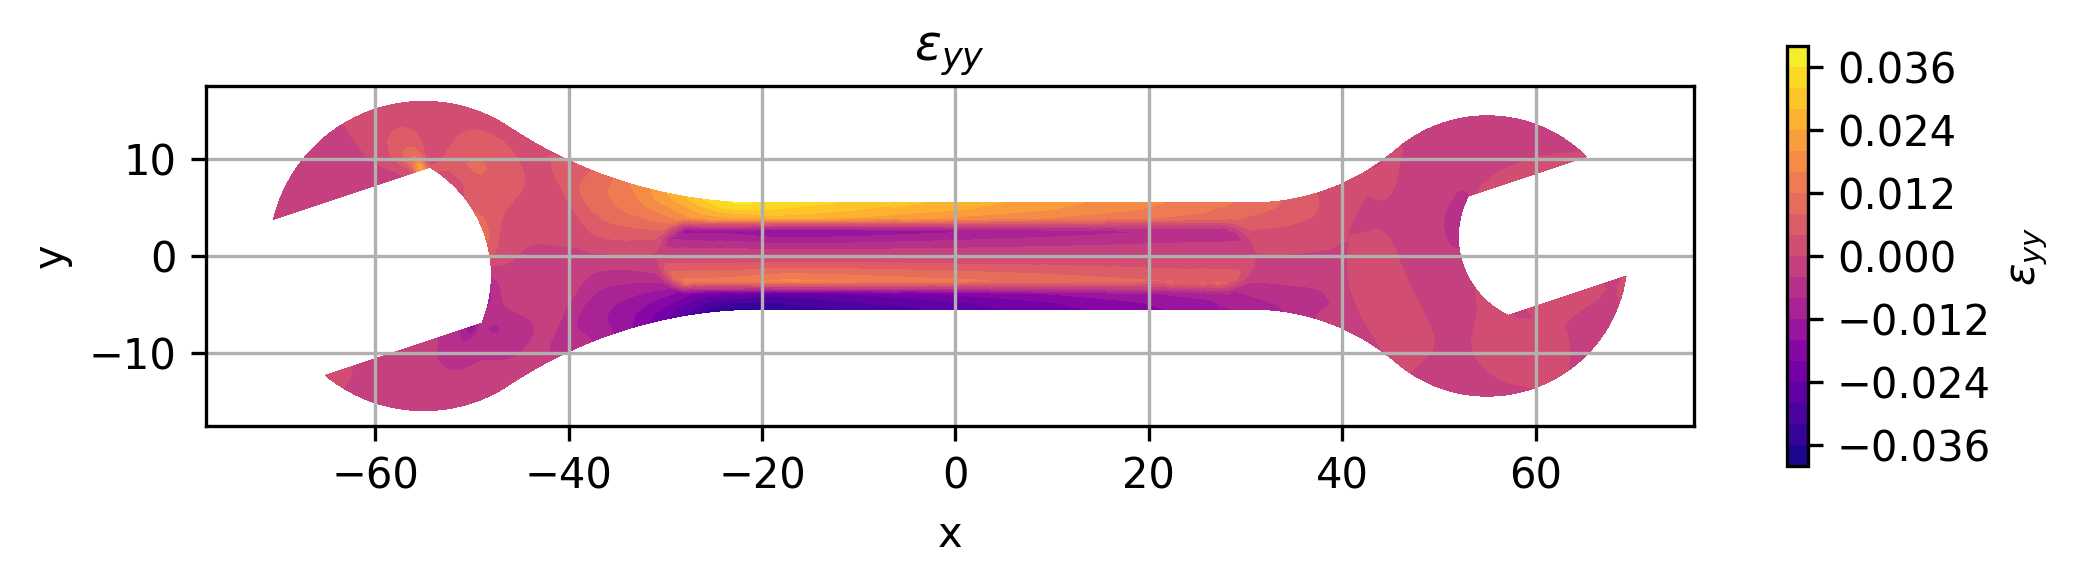
\includegraphics[width=\textwidth]{GRAFICOS/Case b - epsilon_yy.png}
    \caption{Caption}
    \label{fig:von_mises}
  \end{subfigure}
  \caption{Caption}
  \label{fig:analisis_estructural}
\end{figure}


\begin{figure}[H]
  \centering
  \begin{subfigure}[t]{0.49\textwidth}
    \centering
    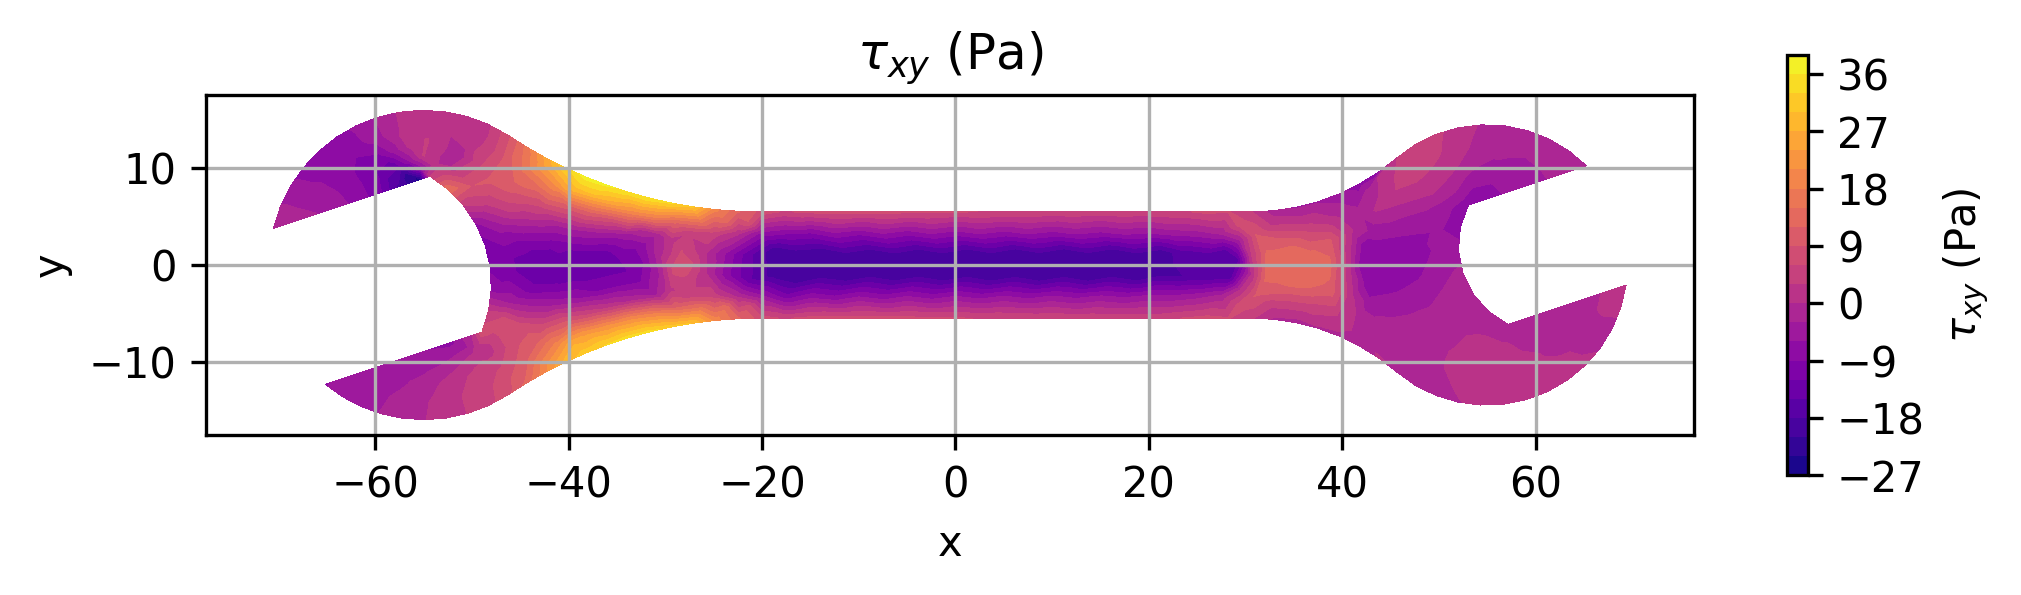
\includegraphics[width=\textwidth]{GRAFICOS/Case b - tau_xy.png}
    \caption{Caption}
    \label{fig:deformada_reacciones}
  \end{subfigure}
  \hfill
  \begin{subfigure}[t]{0.49\textwidth}
    \centering
    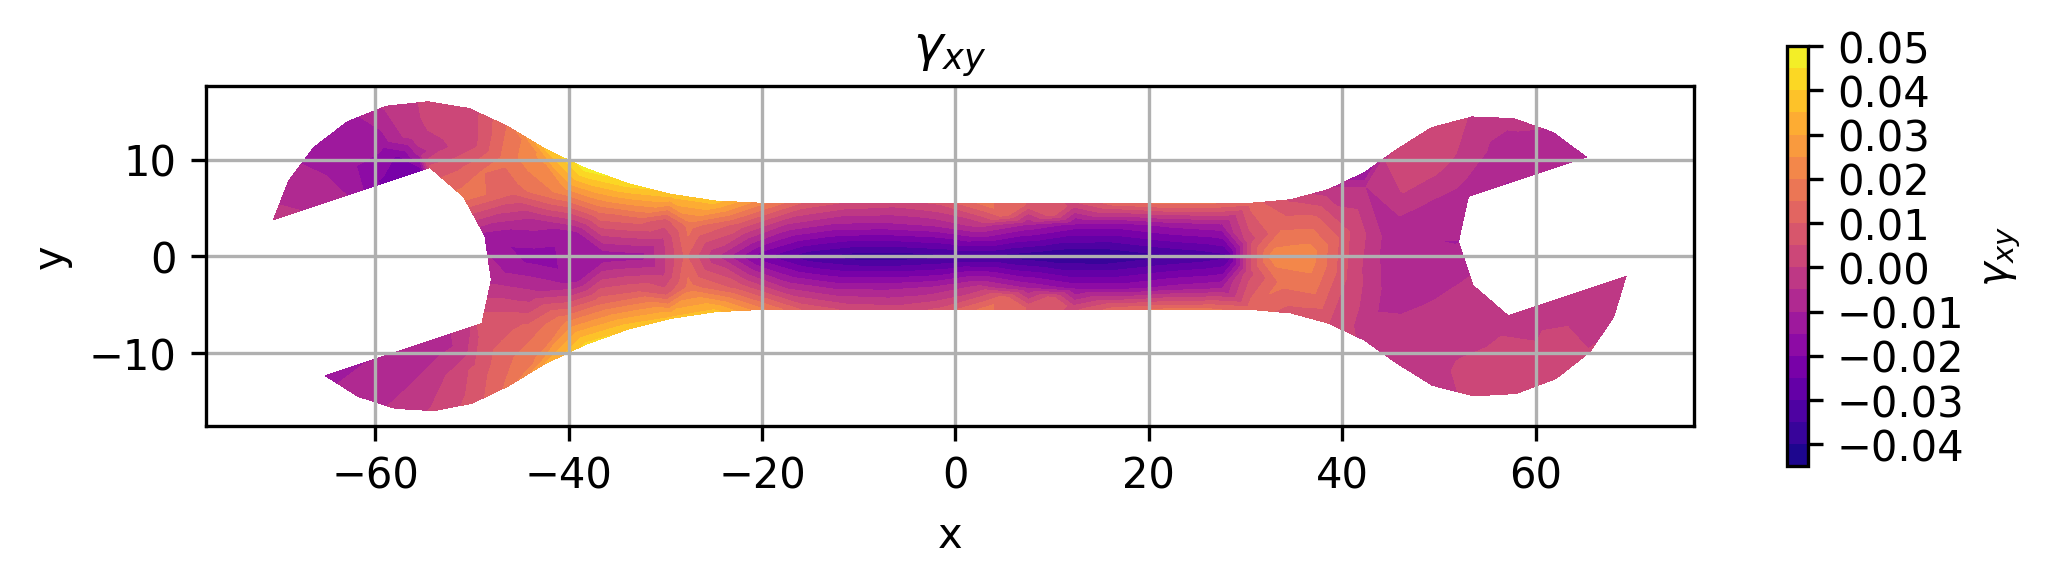
\includegraphics[width=\textwidth]{GRAFICOS/Case b - gamma_xy.png}
    \caption{Caption}
    \label{fig:von_mises}
  \end{subfigure}
  \caption{Caption}
  \label{fig:analisis_estructural}
\end{figure}

\begin{figure}[H]
  \centering
  \begin{subfigure}[t]{0.49\textwidth}
    \centering
    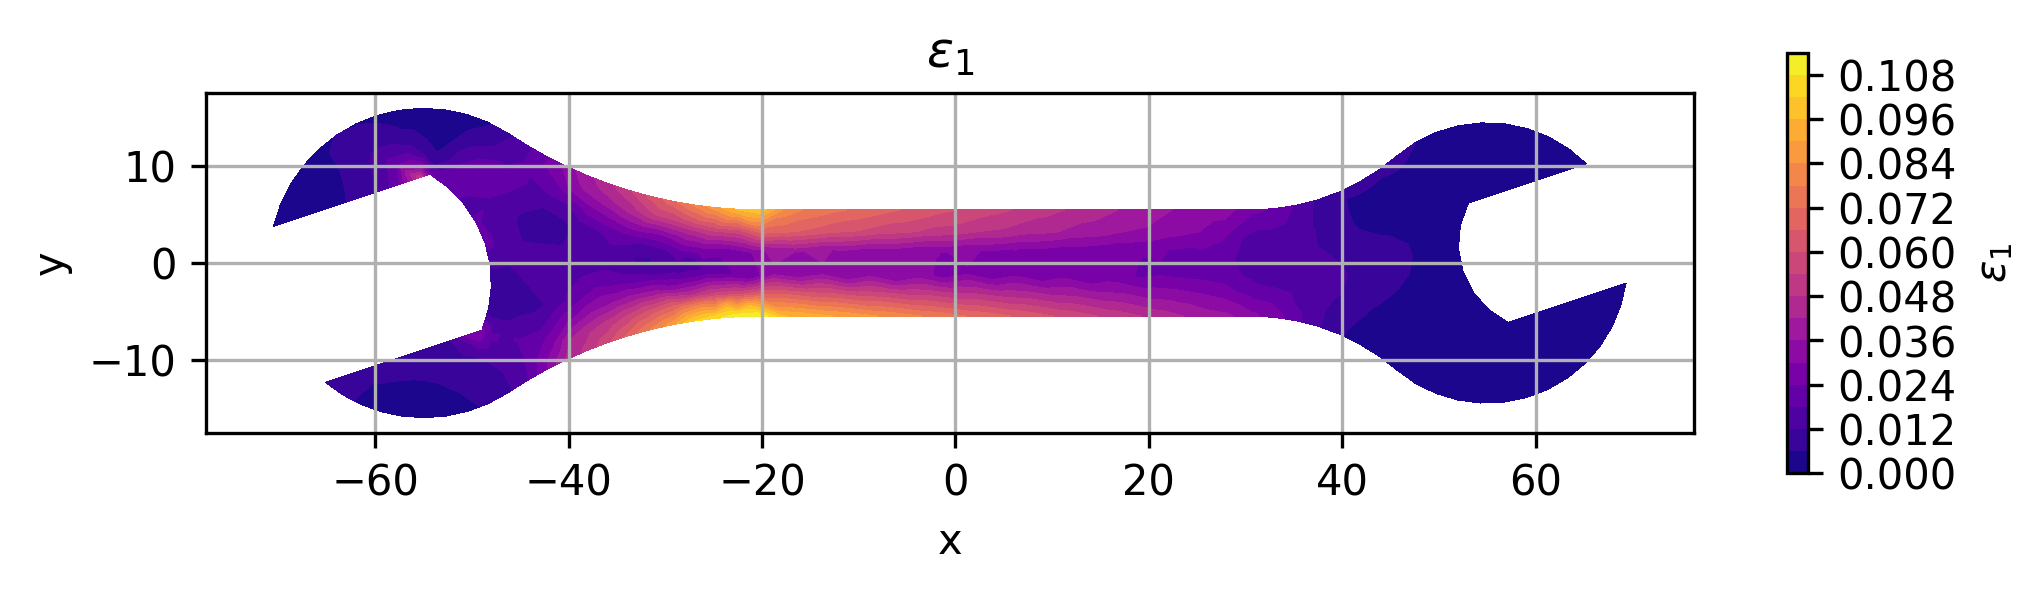
\includegraphics[width=\textwidth]{GRAFICOS/Case b - epsilon_1.png}
    \caption{Caption}
    \label{fig:deformada_reacciones}
  \end{subfigure}
  \hfill
  \begin{subfigure}[t]{0.49\textwidth}
    \centering
    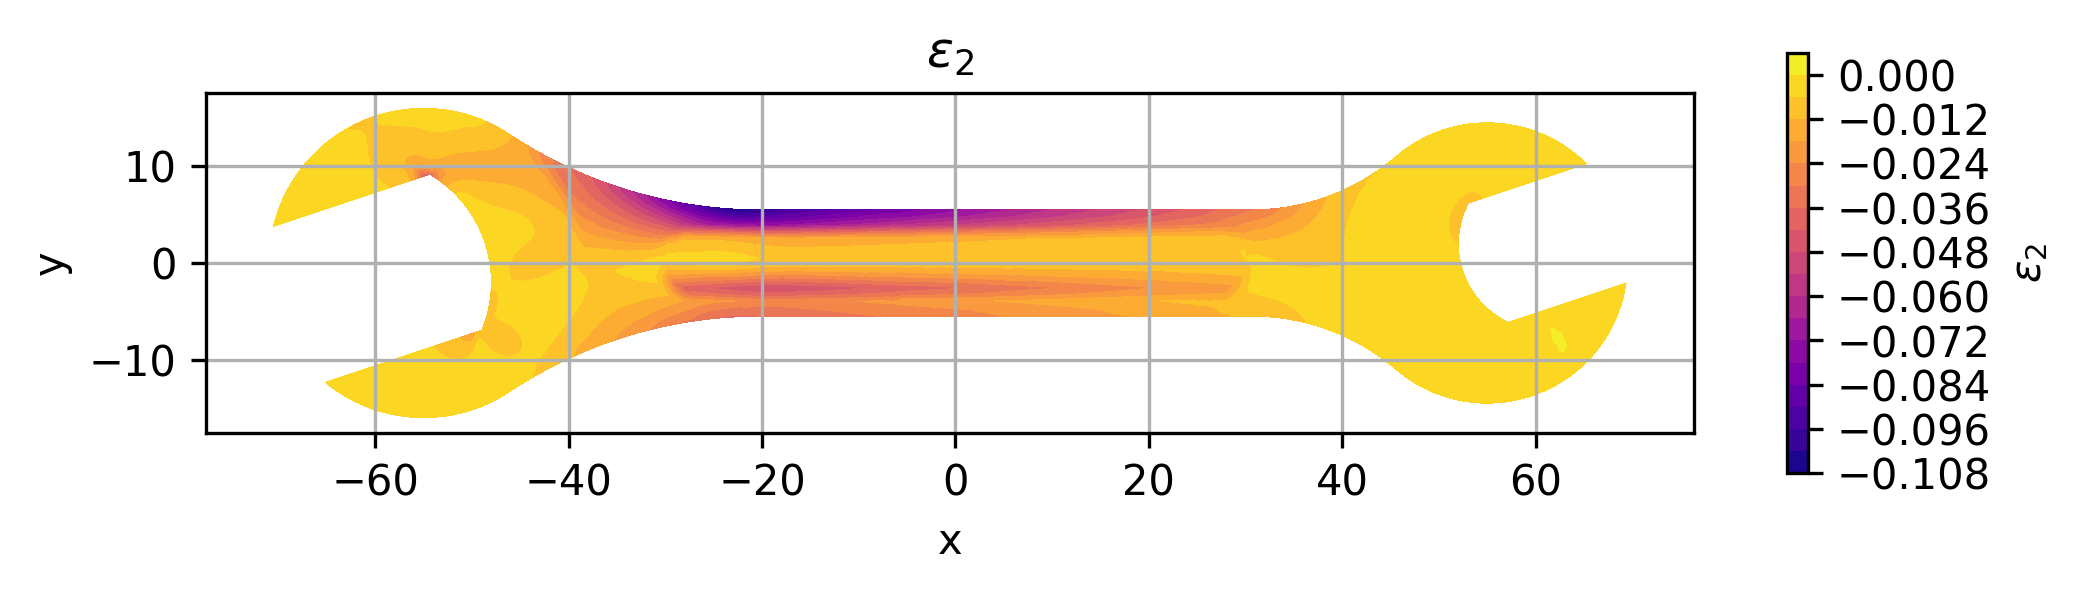
\includegraphics[width=\textwidth]{GRAFICOS/Case b - epsilon_2.png}
    \caption{Caption}
    \label{fig:von_mises}
  \end{subfigure}
  \caption{Caption}
  \label{fig:analisis_estructural}
\end{figure}

\begin{figure}[H]
  \centering
  \begin{subfigure}[t]{0.49\textwidth}
    \centering
    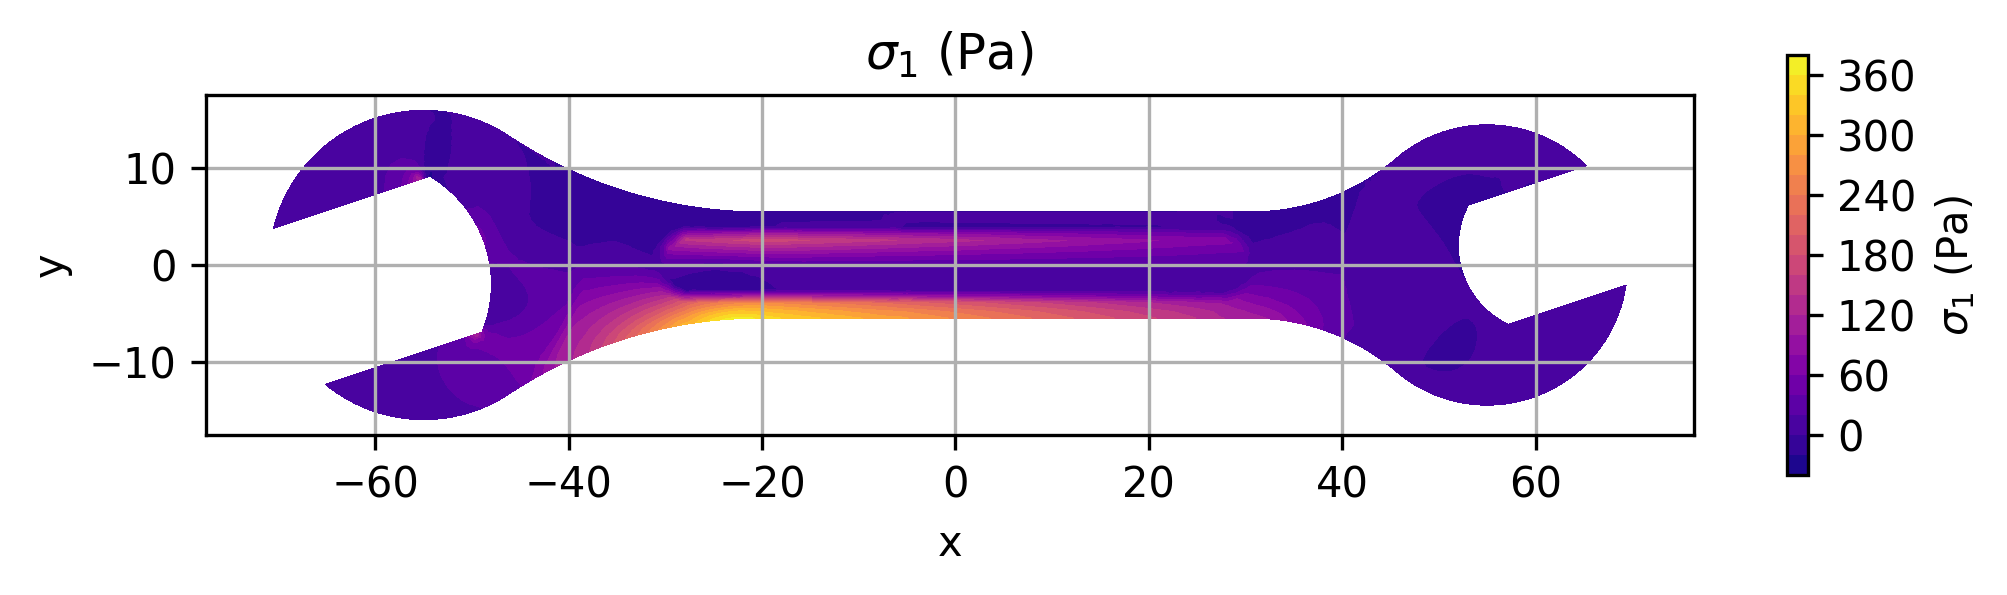
\includegraphics[width=\textwidth]{GRAFICOS/Case b - sigma_1.png}
    \caption{Caption}
    \label{fig:deformada_reacciones}
  \end{subfigure}
  \hfill
  \begin{subfigure}[t]{0.49\textwidth}
    \centering
    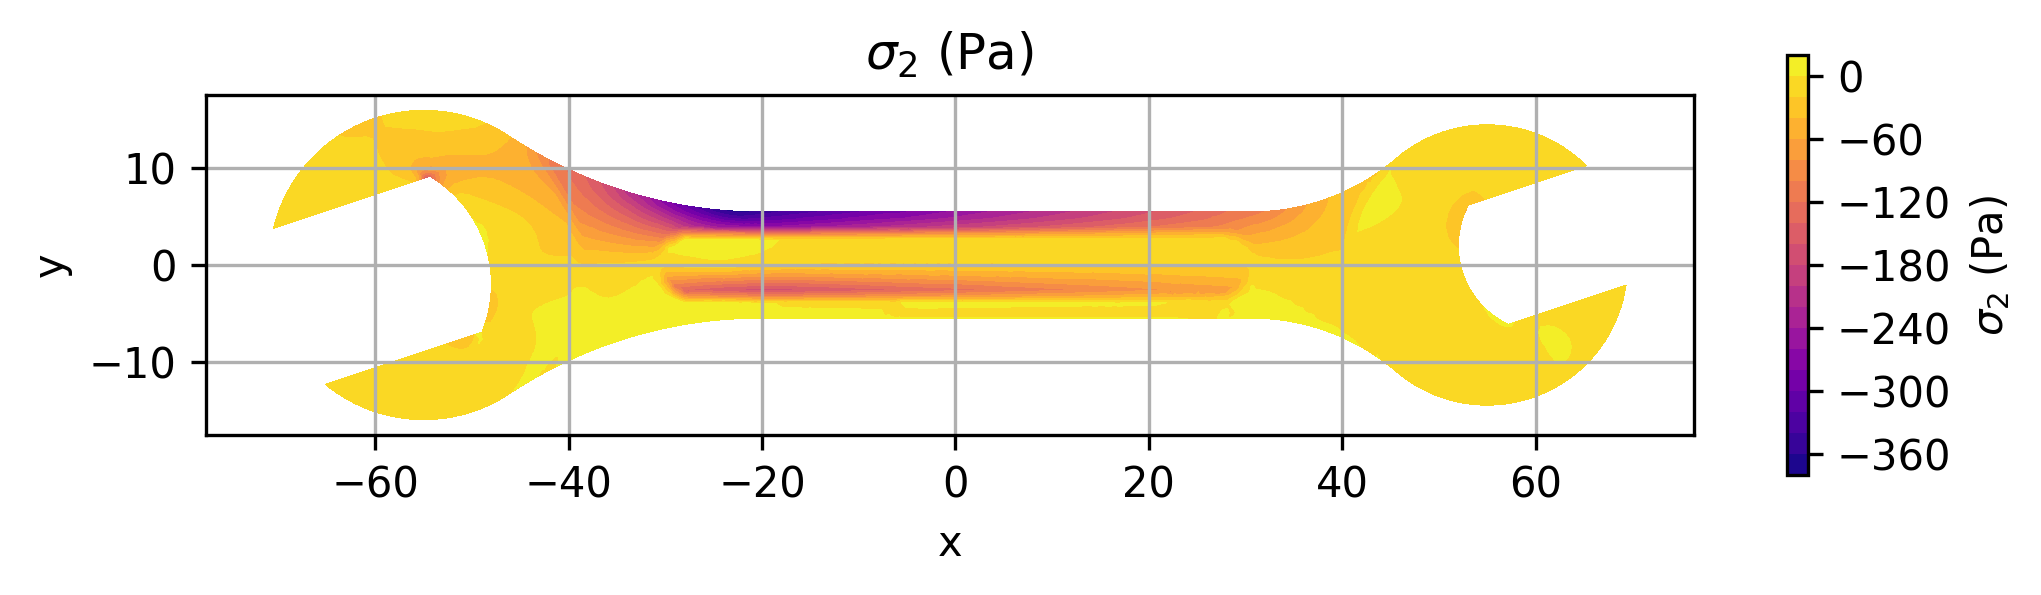
\includegraphics[width=\textwidth]{GRAFICOS/Case b - sigma_2.png}
    \caption{Caption}
    \label{fig:von_mises}
  \end{subfigure}
  \caption{Caption}
  \label{fig:analisis_estructural}
\end{figure}

\section{C case}

\begin{figure}[H]
  \centering
  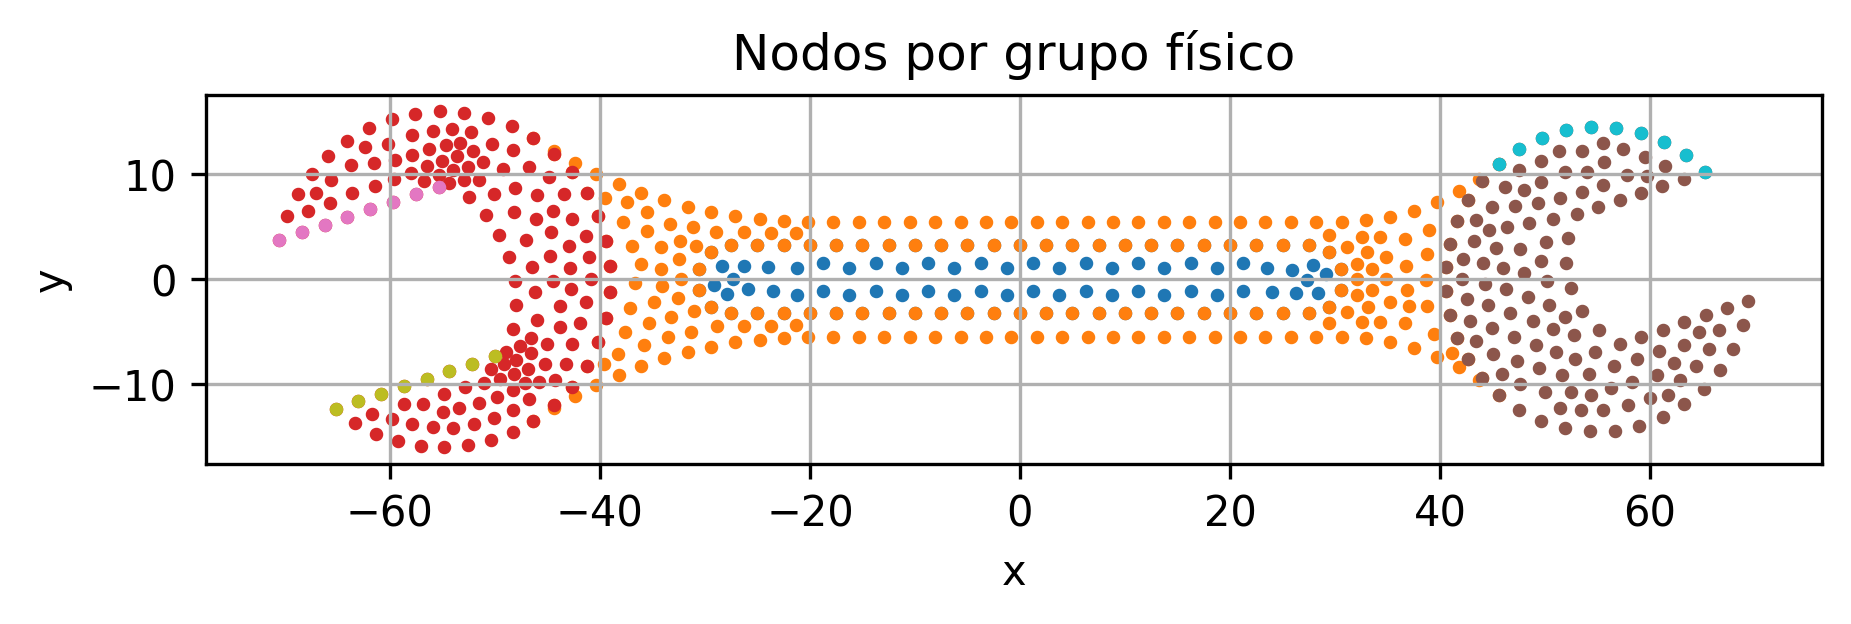
\includegraphics[width=0.8\textwidth]{GRAFICOS/Case c_nodes_por_grupo.png}
  \caption{Caption}
  \label{fig:wrench}
\end{figure}

\begin{figure}[H]
  \centering
  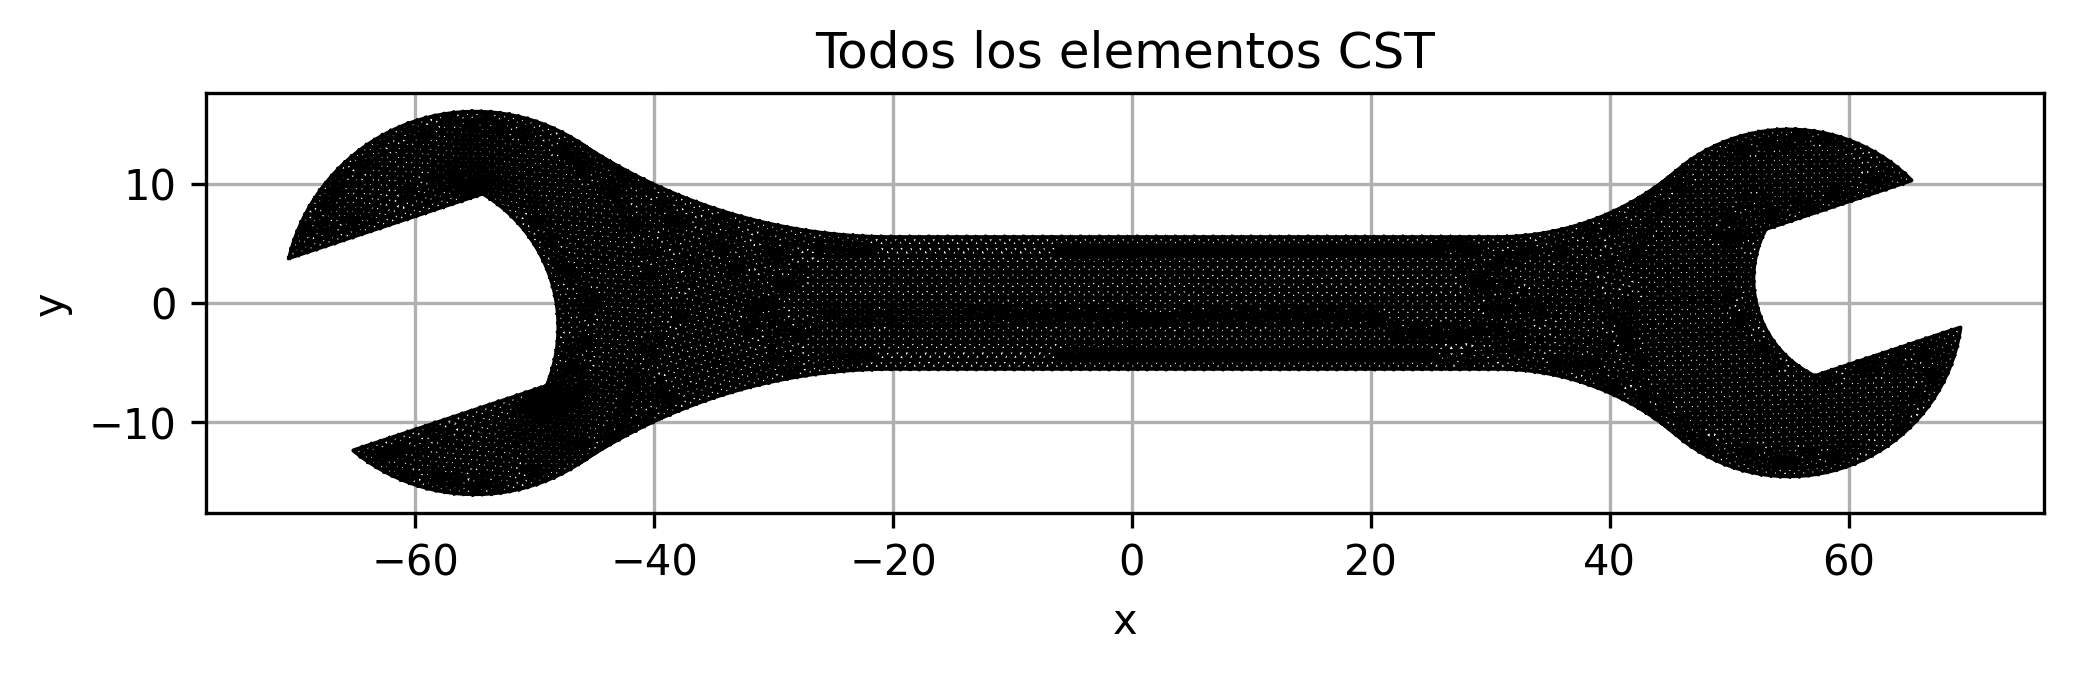
\includegraphics[width=0.8\textwidth]{GRAFICOS/Case c_elementos.png}
  \caption{Caption}
  \label{fig:deformed_shape}
\end{figure}

\begin{figure}[H]
  \centering
  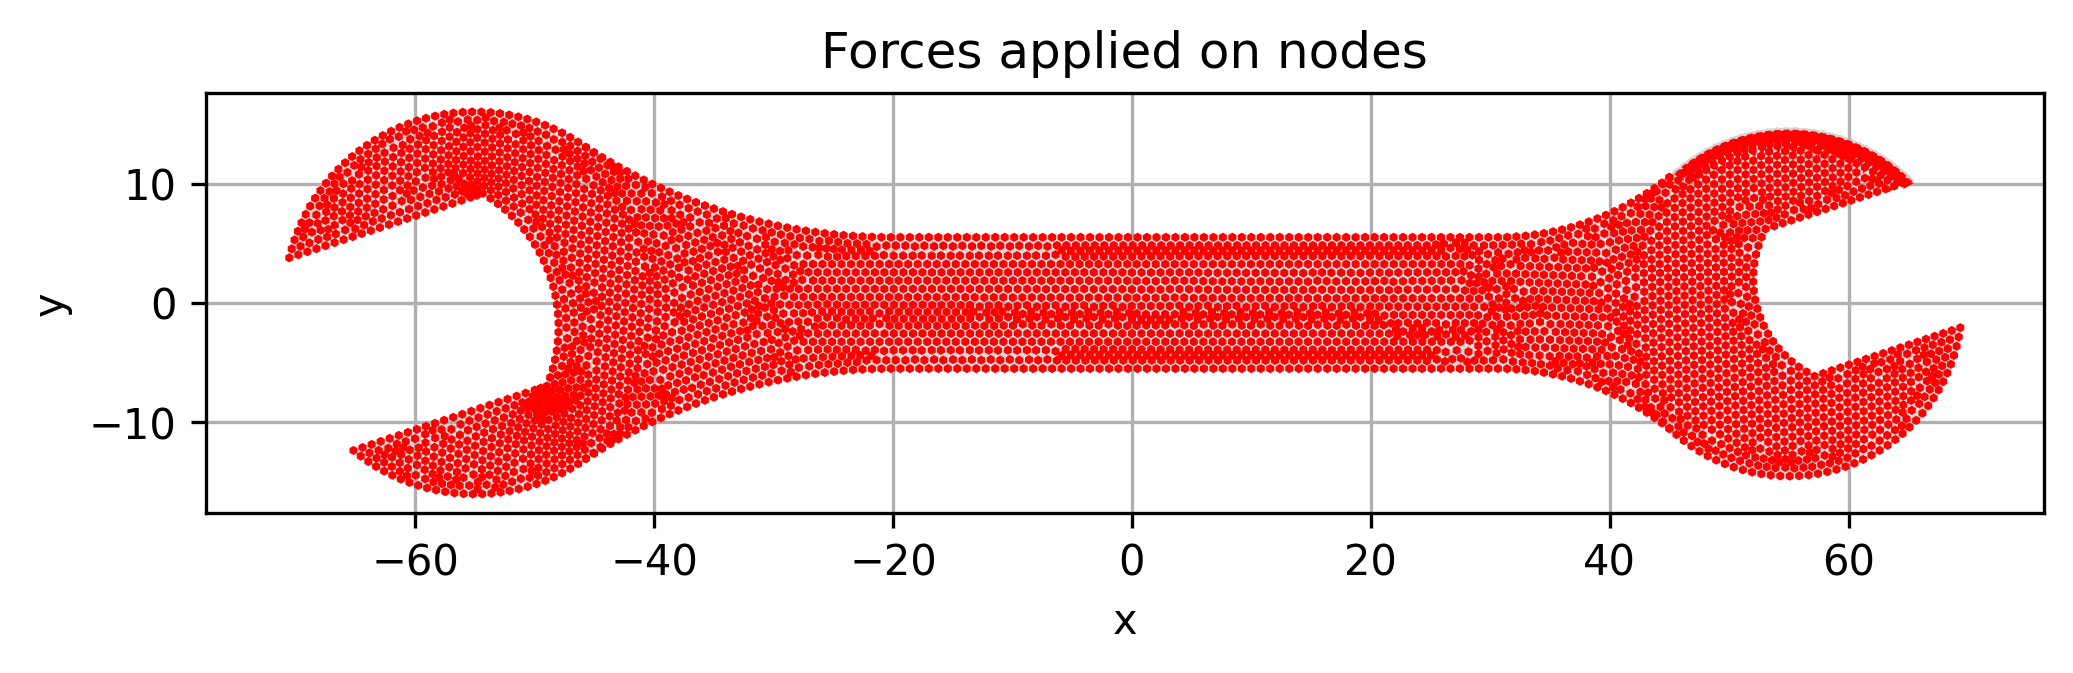
\includegraphics[width=0.8\textwidth]{GRAFICOS/Case c_fuerzas.png}
  \caption{Caption}
  \label{fig:strain}
\end{figure}

\begin{figure}[H]
  \centering
  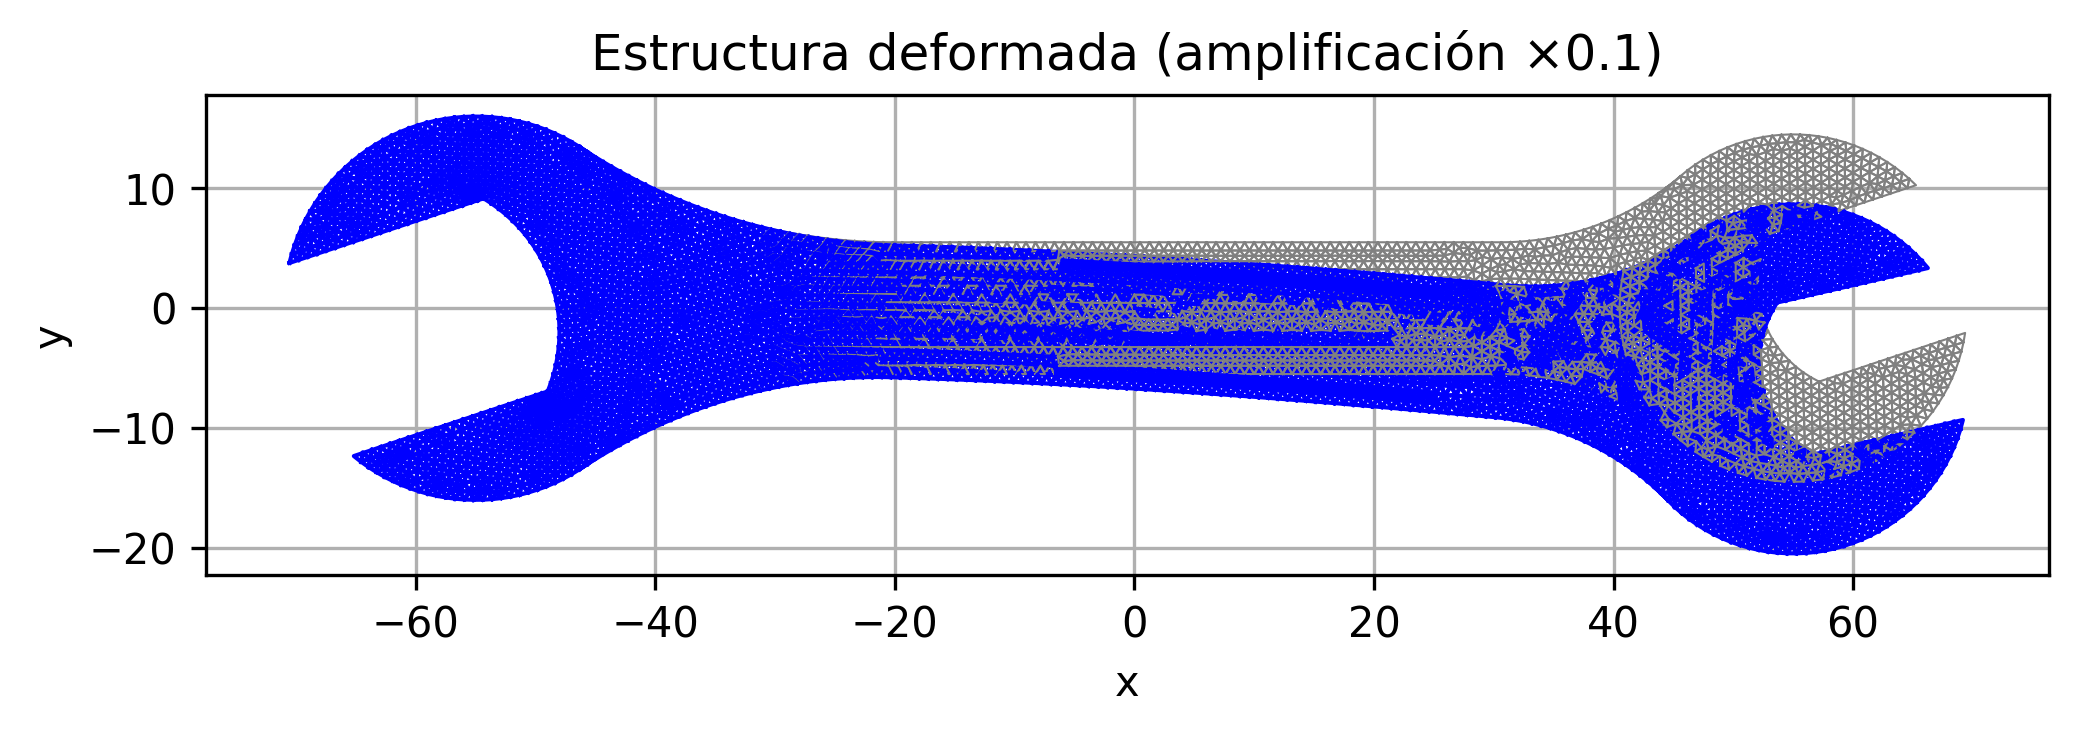
\includegraphics[width=0.8\textwidth]{GRAFICOS/Case c_deformada.png}
  \caption{Caption}
  \label{fig:stress}
\end{figure}

\begin{figure}[H]
  \centering
  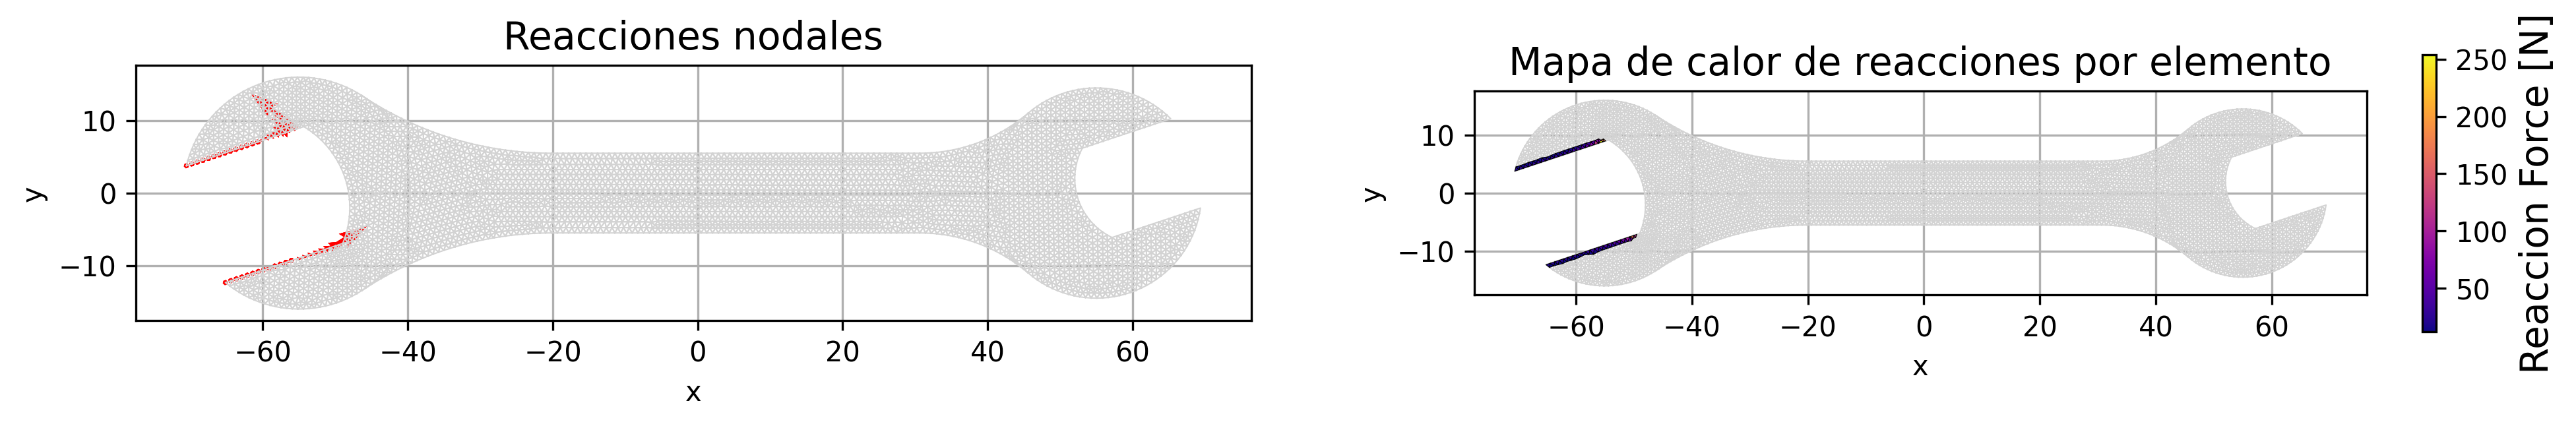
\includegraphics[width=1\textwidth]{GRAFICOS/Case c_deformada_reacciones.png}
  \caption{Caption}
  \label{fig:principal}
\end{figure}

\begin{figure}[H]
  \centering
  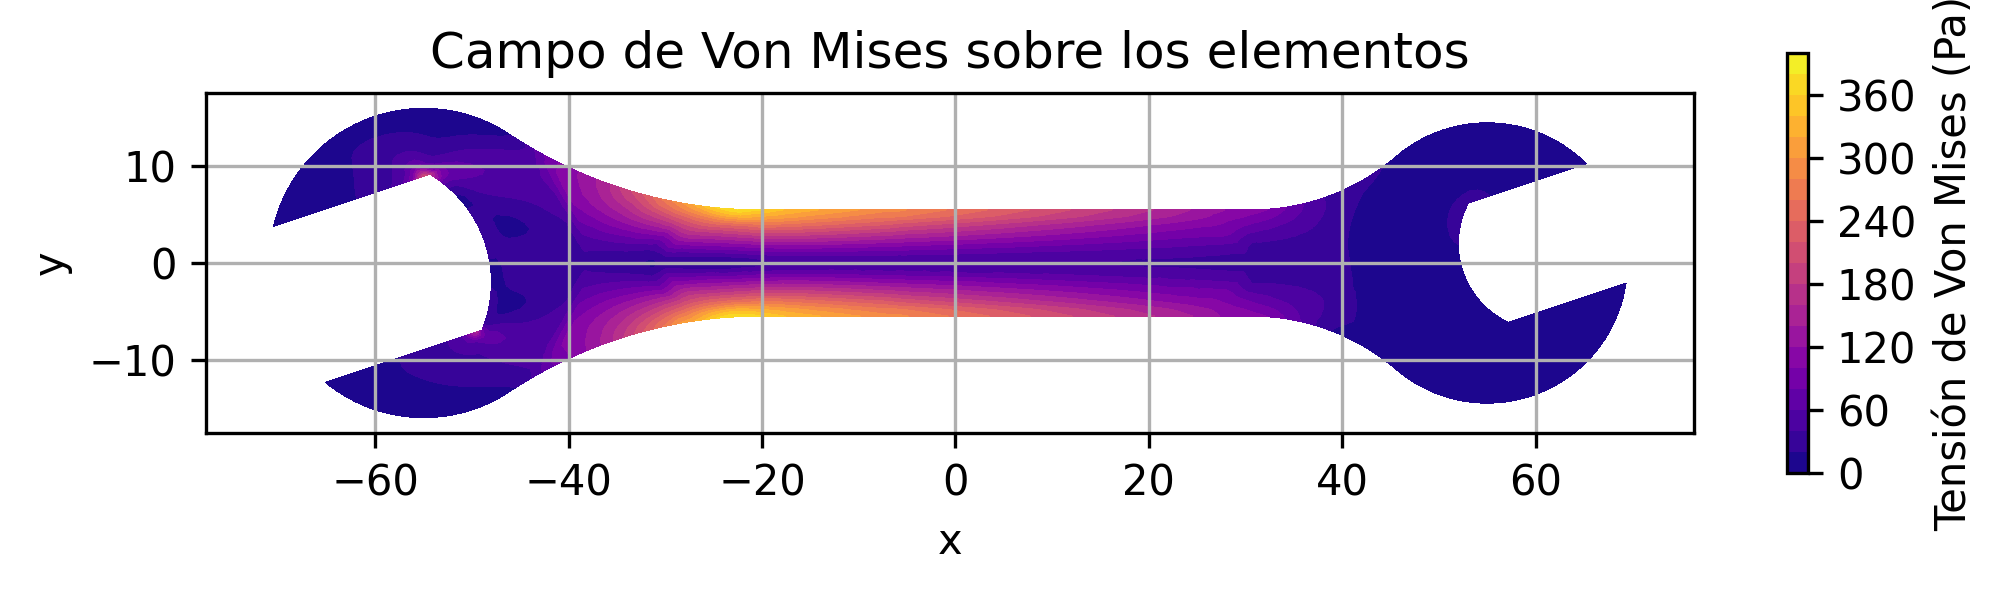
\includegraphics[width=0.8\textwidth]{GRAFICOS/Case c_von_mises.png}
  \caption{Caption}
  \label{fig:principal}
\end{figure}

\begin{figure}[H]
  \centering
  \begin{subfigure}[t]{0.49\textwidth}
    \centering
    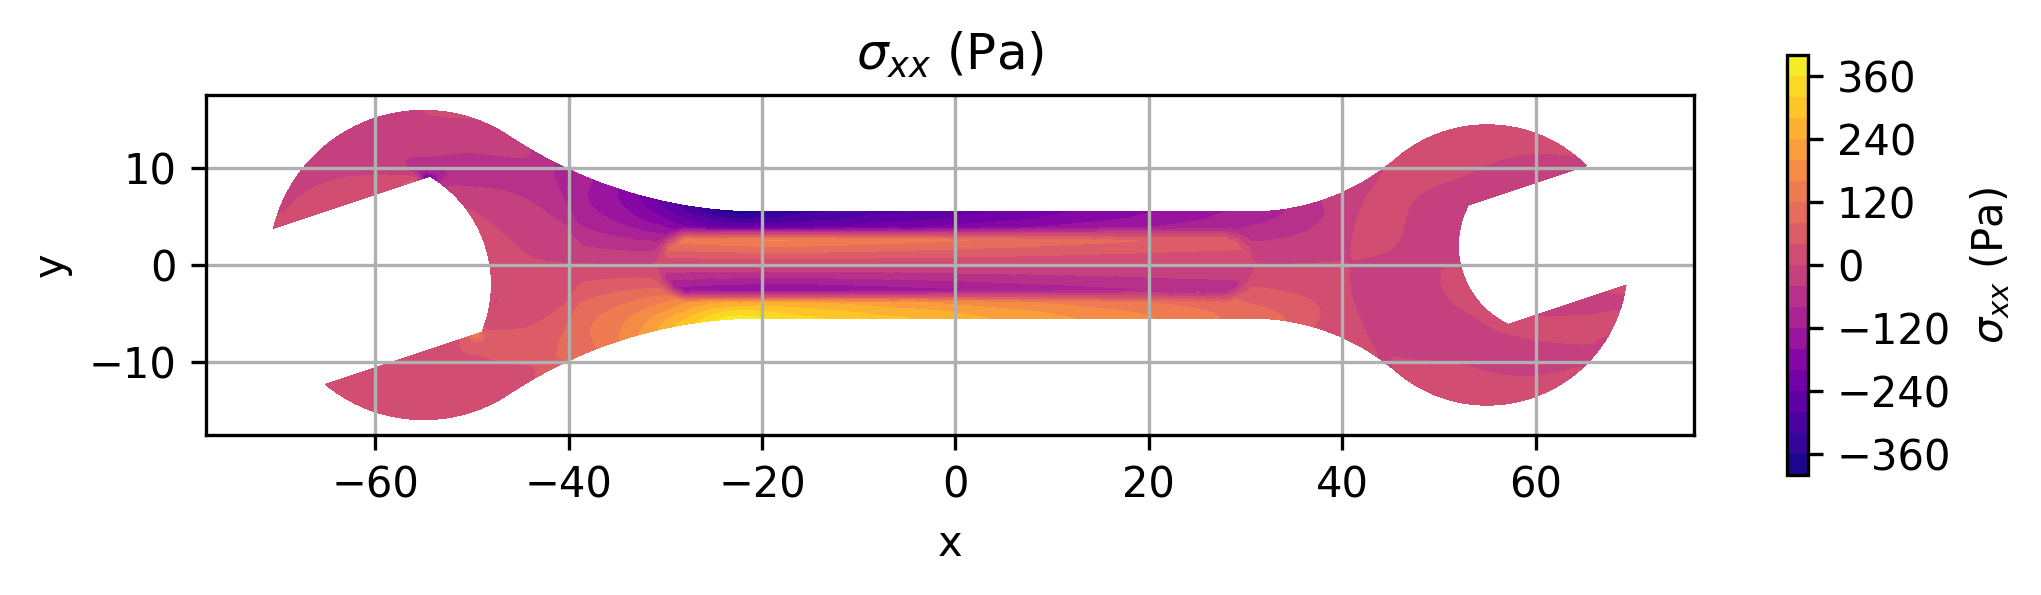
\includegraphics[width=\textwidth]{GRAFICOS/Case c - sigma_xx.png}
    \caption{Caption}
    \label{fig:deformada_reacciones}
  \end{subfigure}
  \hfill
  \begin{subfigure}[t]{0.49\textwidth}
    \centering
    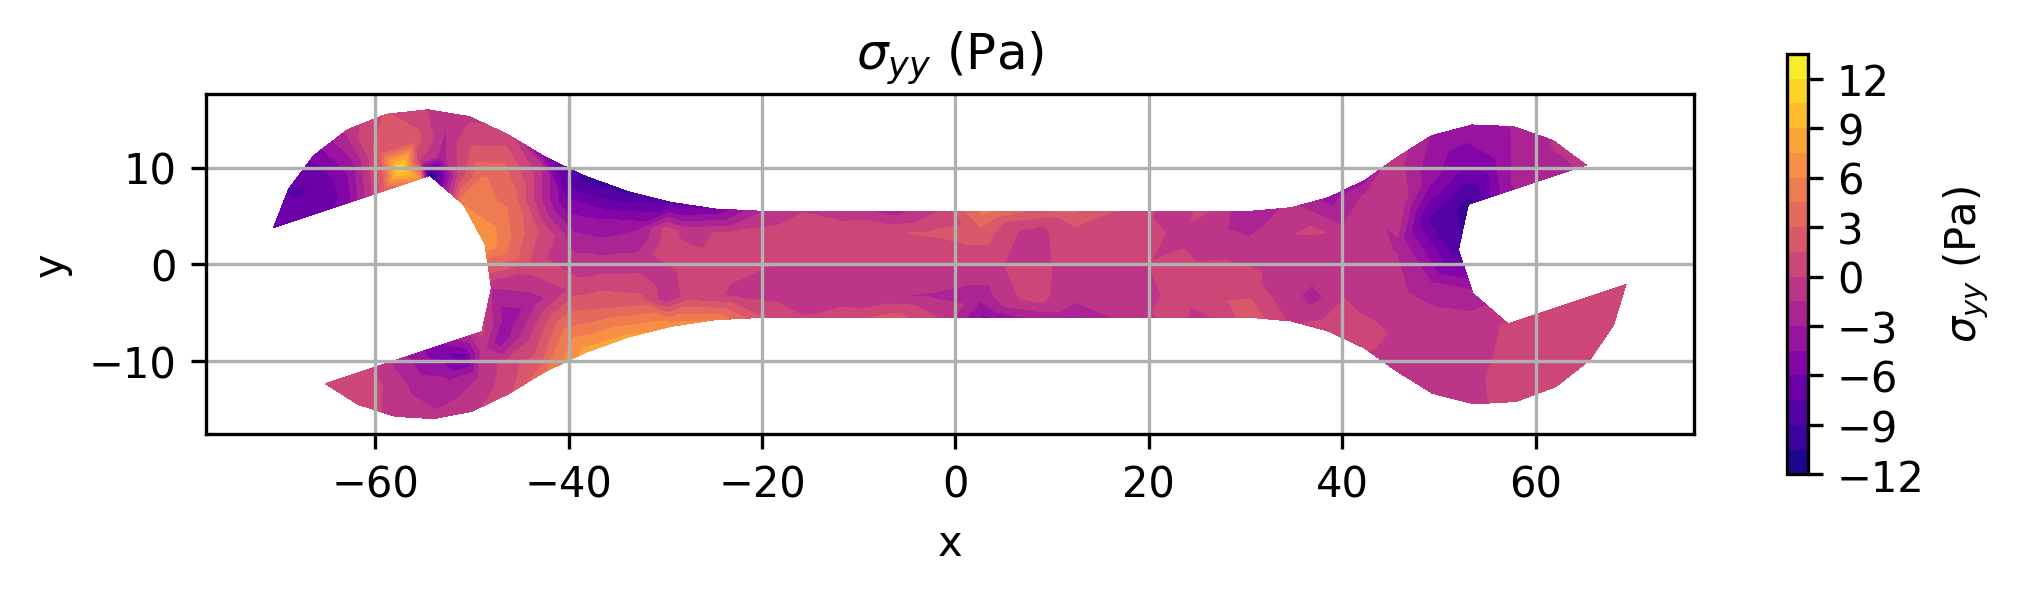
\includegraphics[width=\textwidth]{GRAFICOS/Case c - sigma_yy.png}
    \caption{Caption}
    \label{fig:von_mises}
  \end{subfigure}
  \caption{Caption}
  \label{fig:analisis_estructural}
\end{figure}

\begin{figure}[H]
  \centering
  \begin{subfigure}[t]{0.49\textwidth}
    \centering
    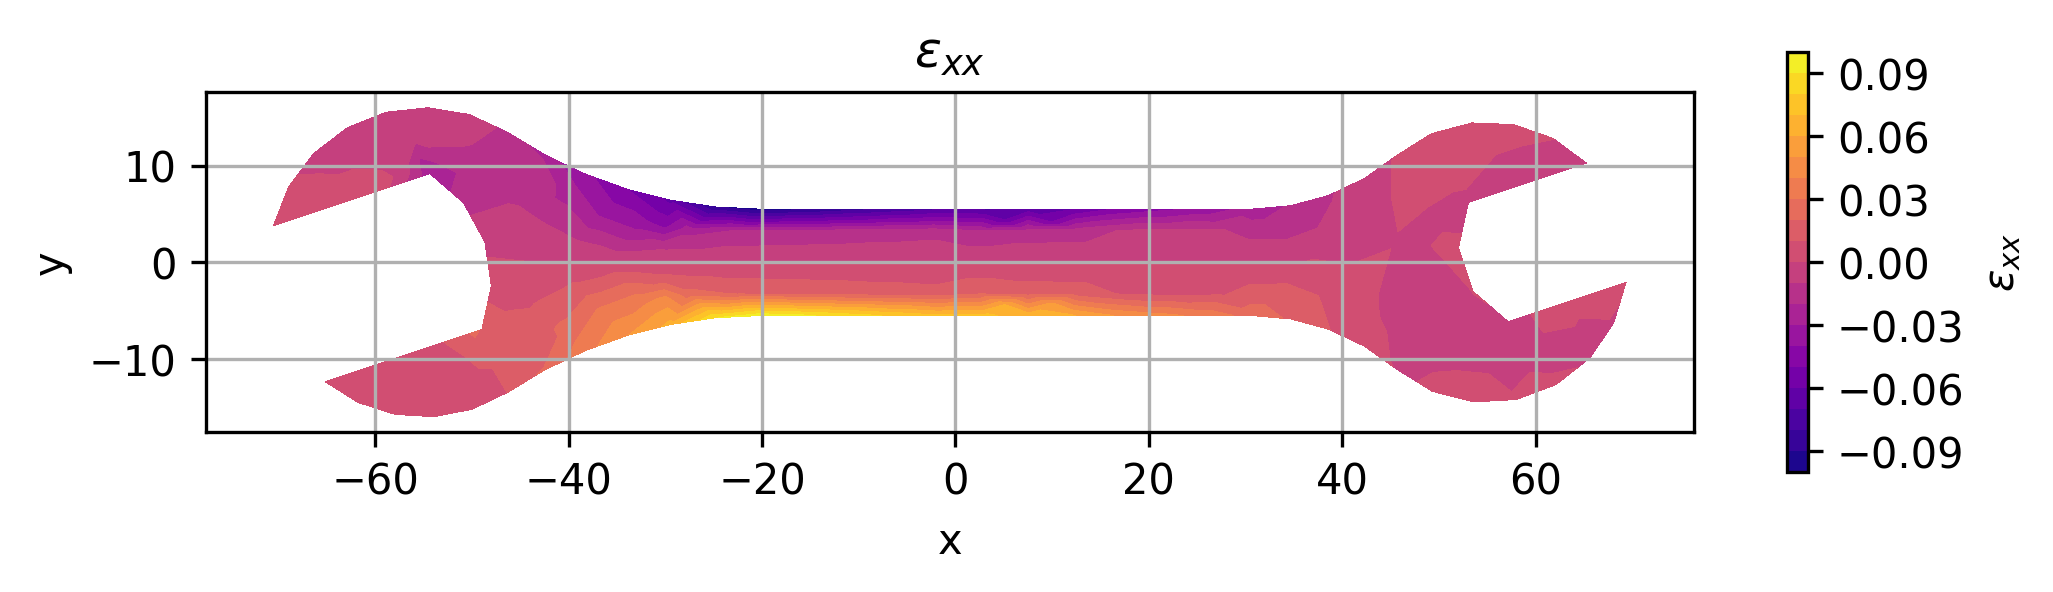
\includegraphics[width=\textwidth]{GRAFICOS/Case c - epsilon_xx.png}
    \caption{Caption}
    \label{fig:deformada_reacciones}
  \end{subfigure}
  \hfill
  \begin{subfigure}[t]{0.49\textwidth}
    \centering
    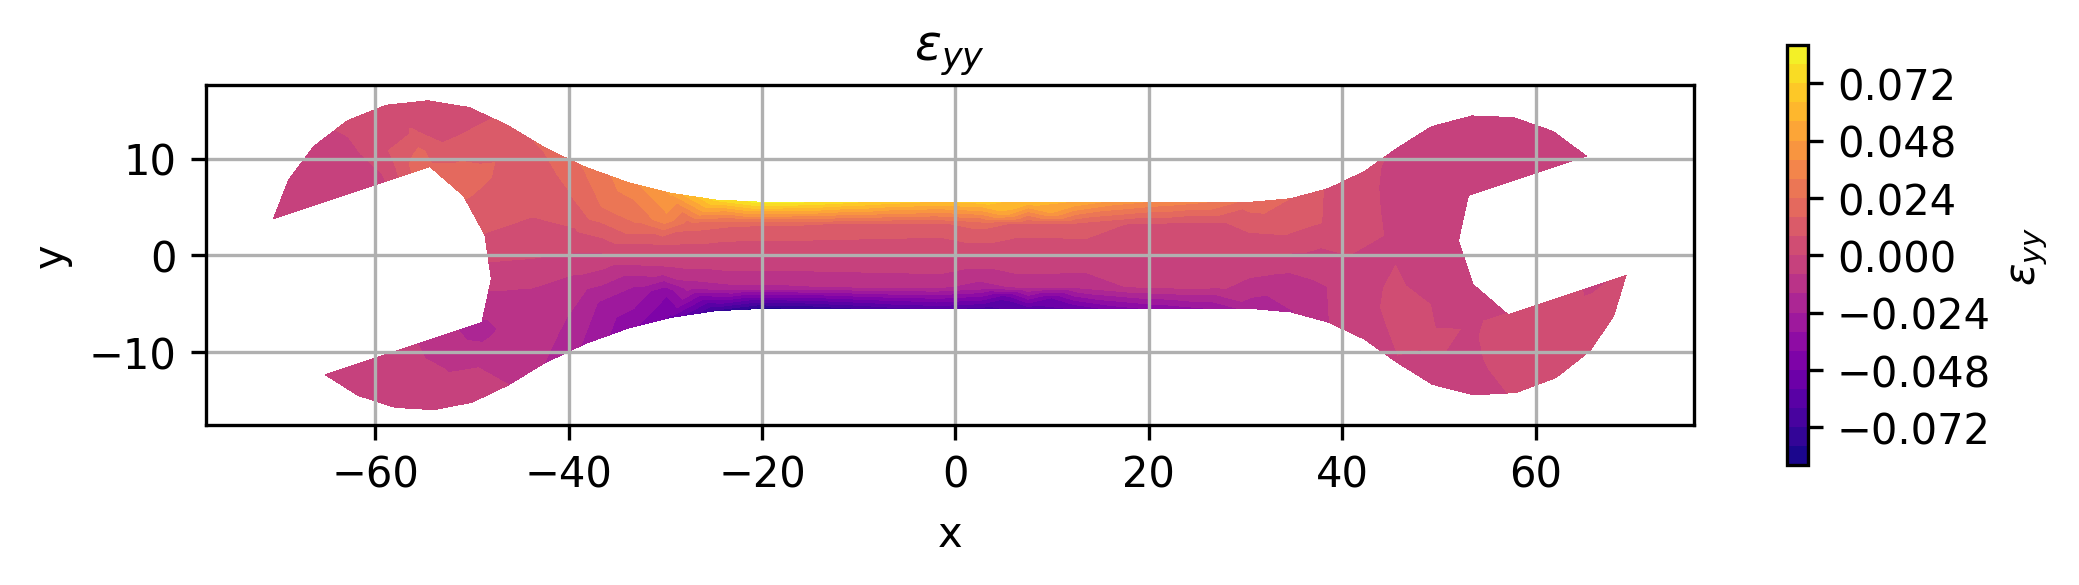
\includegraphics[width=\textwidth]{GRAFICOS/Case c - epsilon_yy.png}
    \caption{Caption}
    \label{fig:von_mises}
  \end{subfigure}
  \caption{Caption}
  \label{fig:analisis_estructural}
\end{figure}


\begin{figure}[H]
  \centering
  \begin{subfigure}[t]{0.49\textwidth}
    \centering
    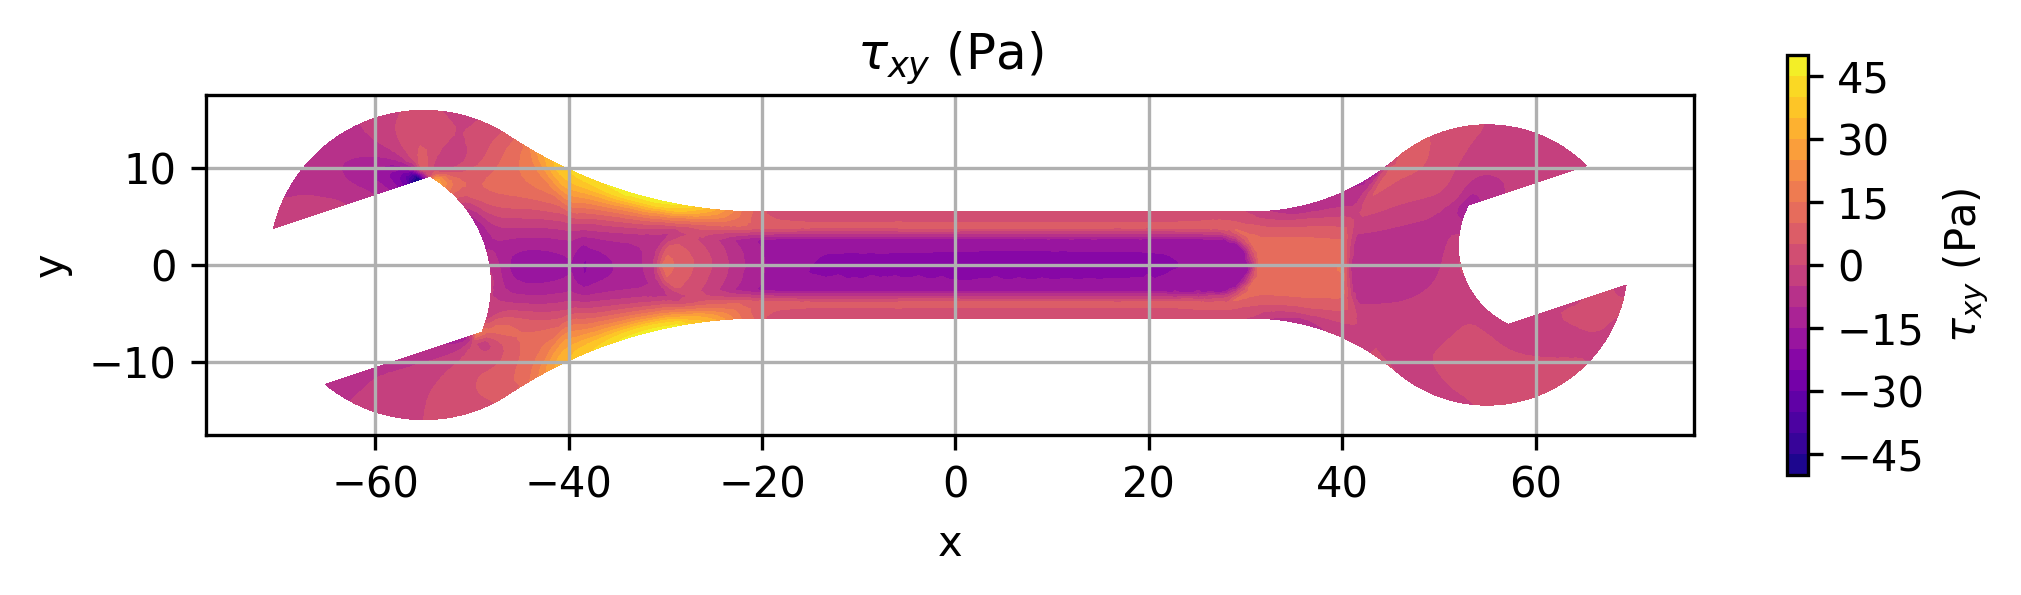
\includegraphics[width=\textwidth]{GRAFICOS/Case c - tau_xy.png}
    \caption{Caption}
    \label{fig:deformada_reacciones}
  \end{subfigure}
  \hfill
  \begin{subfigure}[t]{0.49\textwidth}
    \centering
    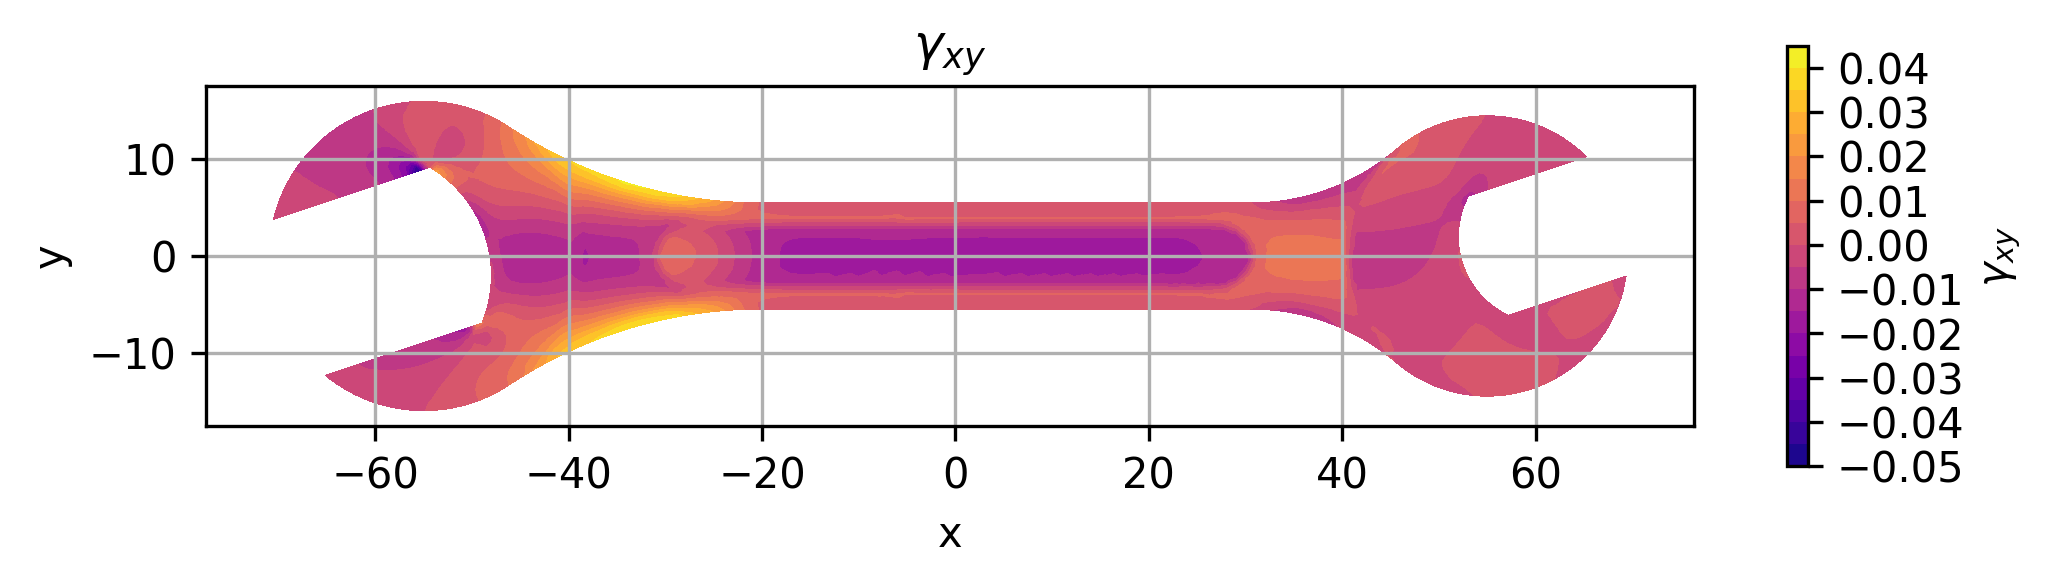
\includegraphics[width=\textwidth]{GRAFICOS/Case c - gamma_xy.png}
    \caption{Caption}
    \label{fig:von_mises}
  \end{subfigure}
  \caption{Caption}
  \label{fig:analisis_estructural}
\end{figure}

\begin{figure}[H]
  \centering
  \begin{subfigure}[t]{0.49\textwidth}
    \centering
    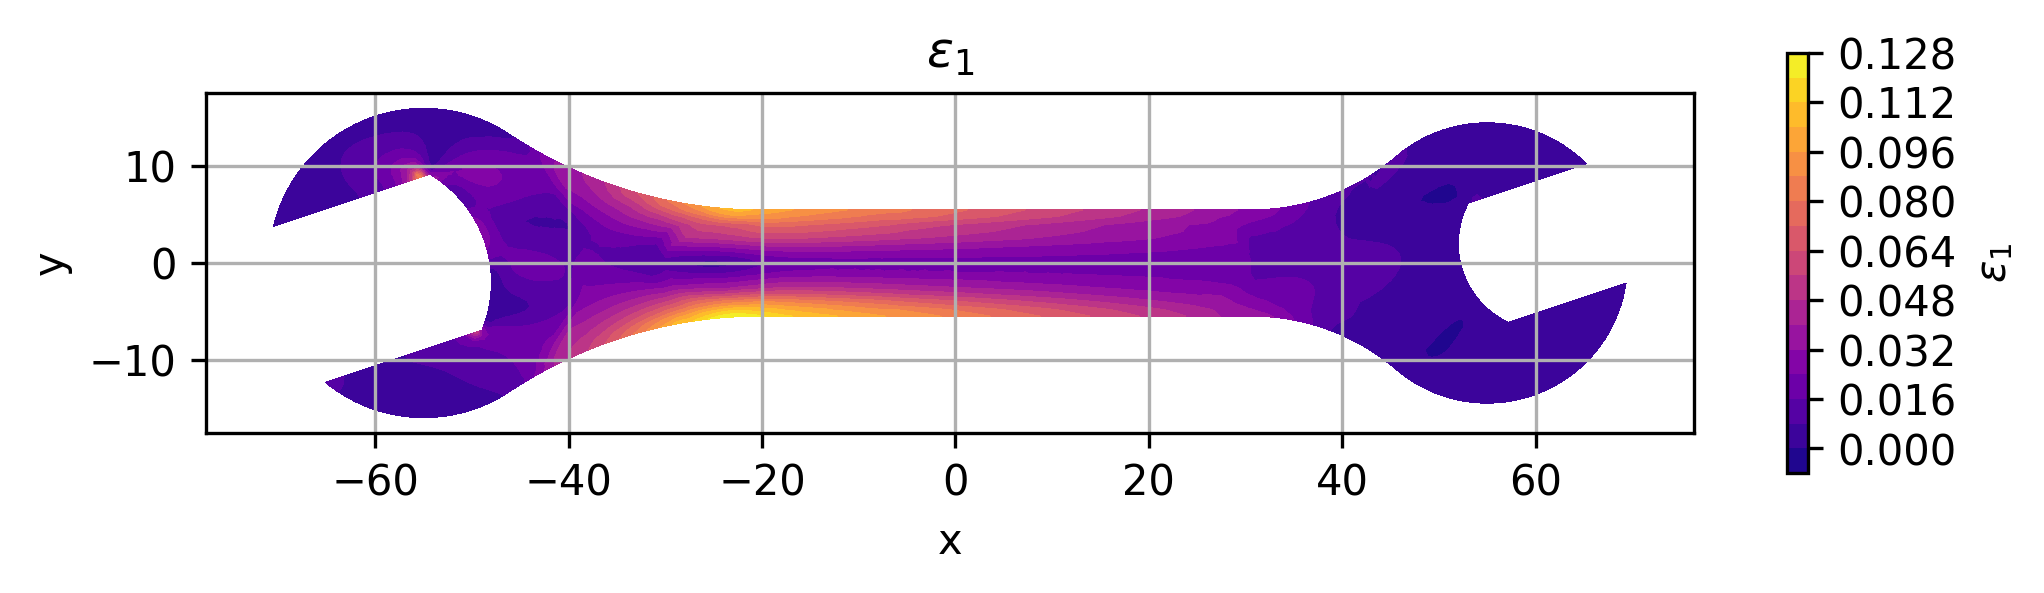
\includegraphics[width=\textwidth]{GRAFICOS/Case c - epsilon_1.png}
    \caption{Caption}
    \label{fig:deformada_reacciones}
  \end{subfigure}
  \hfill
  \begin{subfigure}[t]{0.49\textwidth}
    \centering
    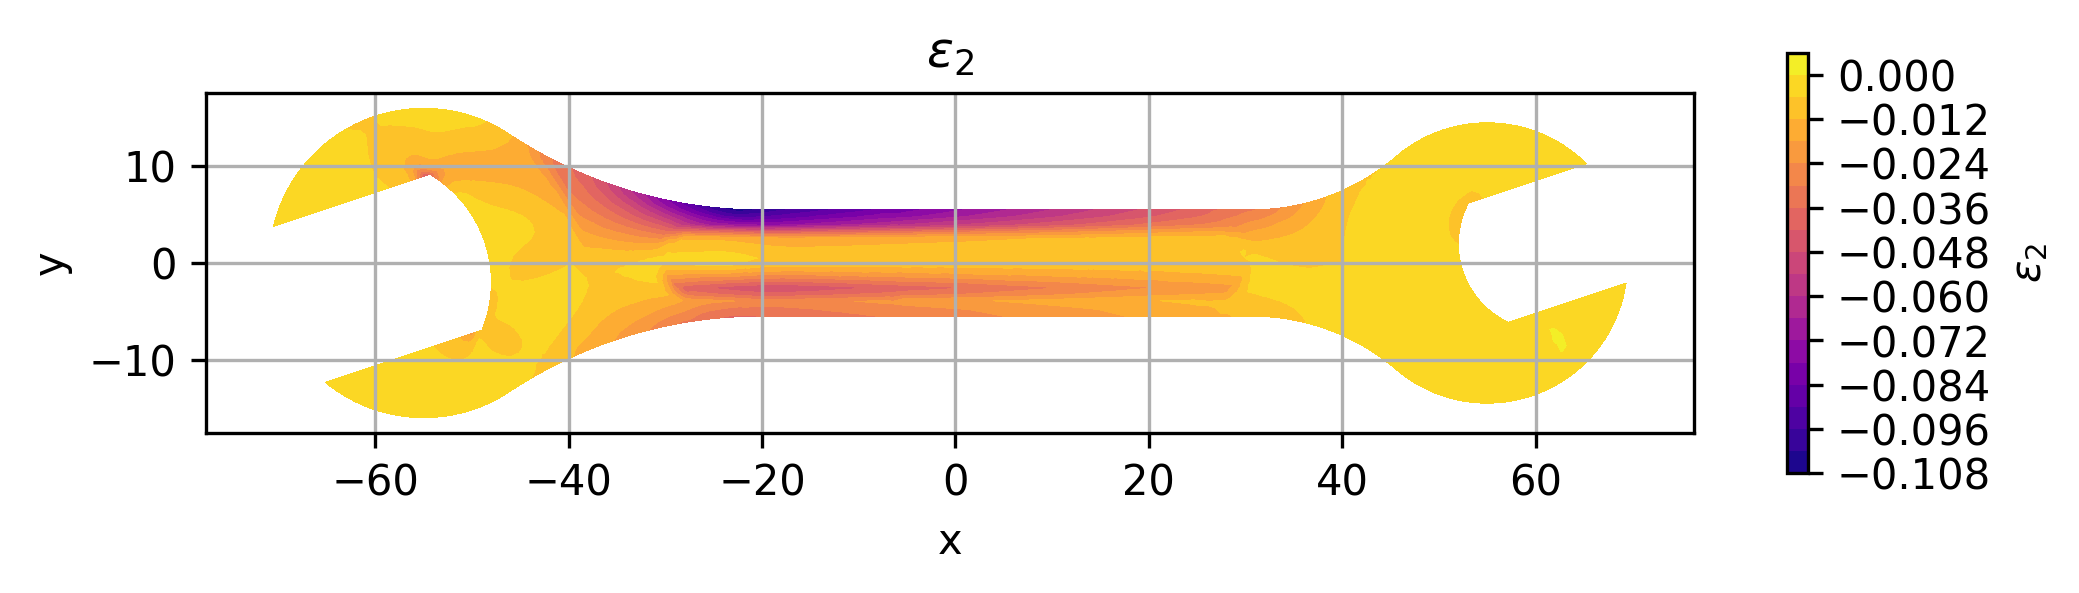
\includegraphics[width=\textwidth]{GRAFICOS/Case c - epsilon_2.png}
    \caption{Caption}
    \label{fig:von_mises}
  \end{subfigure}
  \caption{Caption}
  \label{fig:analisis_estructural}
\end{figure}

\begin{figure}[H]
  \centering
  \begin{subfigure}[t]{0.49\textwidth}
    \centering
    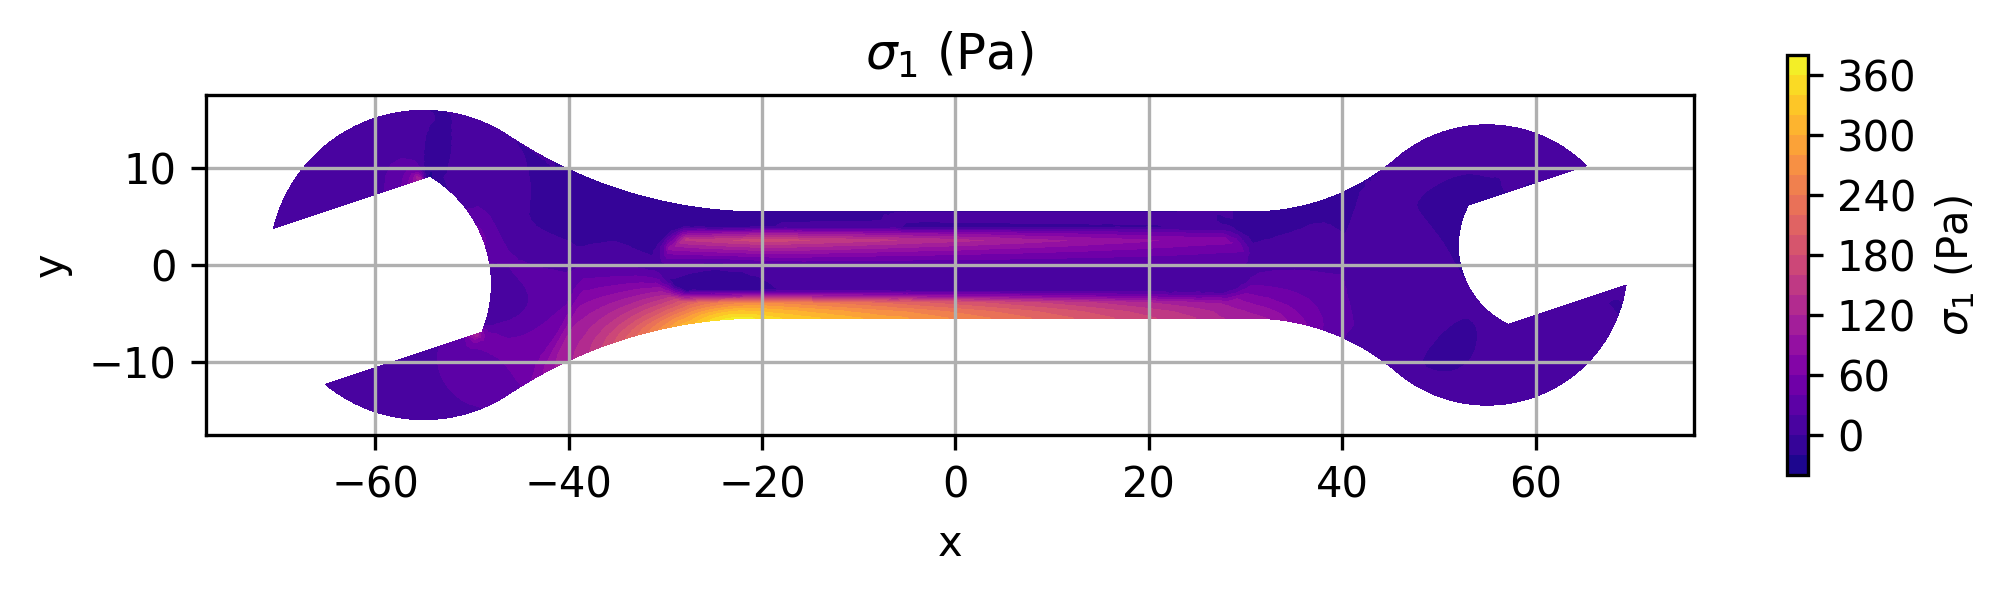
\includegraphics[width=\textwidth]{GRAFICOS/Case c - sigma_1.png}
    \caption{Caption}
    \label{fig:deformada_reacciones}
  \end{subfigure}
  \hfill
  \begin{subfigure}[t]{0.49\textwidth}
    \centering
    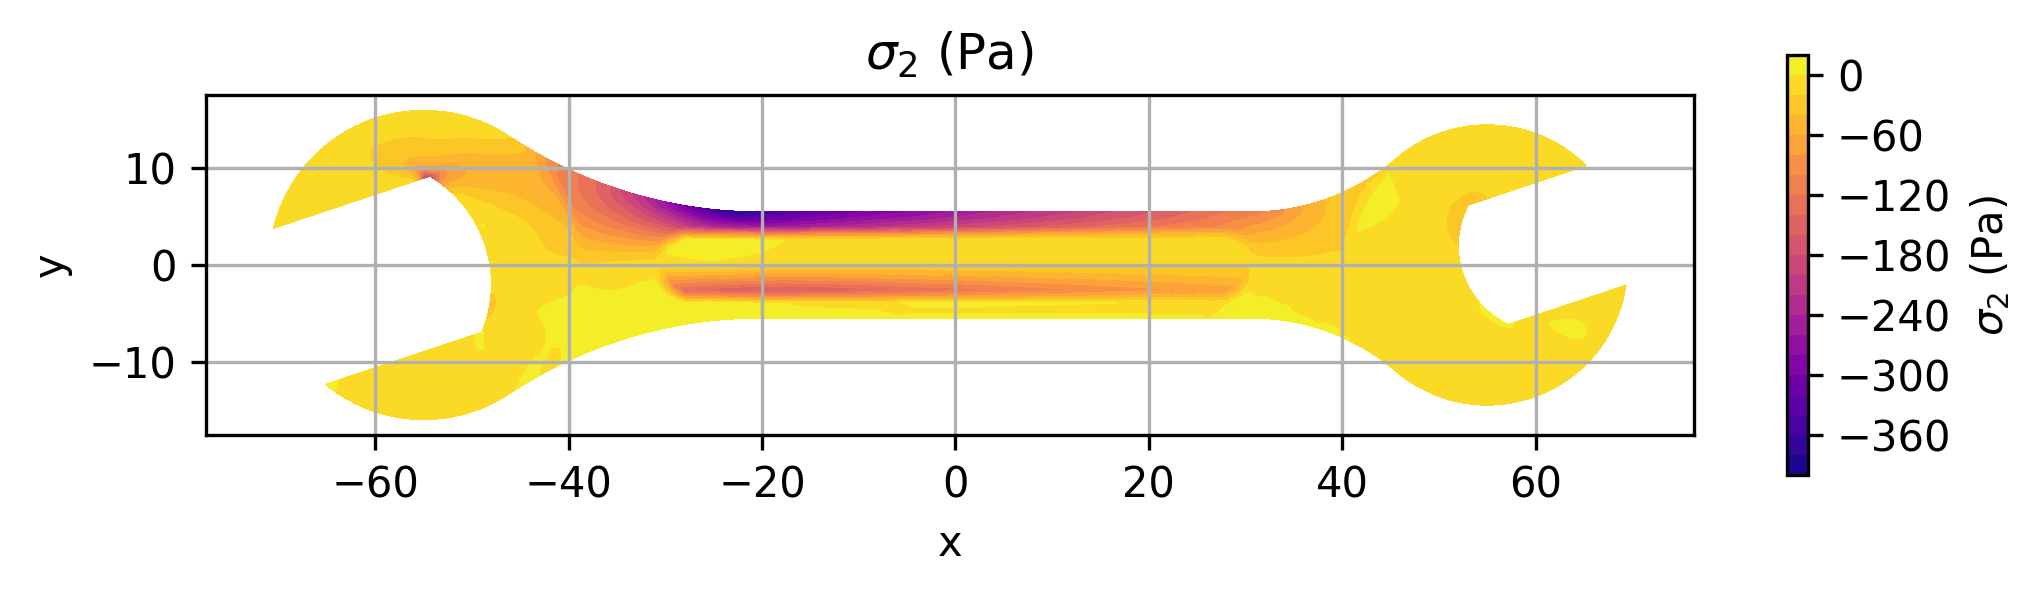
\includegraphics[width=\textwidth]{GRAFICOS/Case c - sigma_2.png}
    \caption{Caption}
    \label{fig:von_mises}
  \end{subfigure}
  \caption{Caption}
  \label{fig:analisis_estructural}
\end{figure}

\section{D case, only self weight}

\begin{figure}[H]
  \centering
  \includegraphics[width=0.8\textwidth]{GRAFICOS/Case d_nodes_por_grupo.png}
  \caption{Caption}
  \label{fig:wrench}
\end{figure}

\begin{figure}[H]
  \centering
  \includegraphics[width=0.8\textwidth]{GRAFICOS/Case d_elementos.png}
  \caption{Caption}
  \label{fig:deformed_shape}
\end{figure}

\begin{figure}[H]
  \centering
  \includegraphics[width=0.8\textwidth]{GRAFICOS/Case d_fuerzas.png}
  \caption{Caption}
  \label{fig:strain}
\end{figure}

\begin{figure}[H]
  \centering
  \includegraphics[width=0.8\textwidth]{GRAFICOS/Case d_deformada.png}
  \caption{Caption}
  \label{fig:stress}
\end{figure}

\begin{figure}[H]
  \centering
  \includegraphics[width=1\textwidth]{GRAFICOS/Case d_deformada_reacciones.png}
  \caption{Caption}
  \label{fig:principal}
\end{figure}

\begin{figure}[H]
  \centering
  \includegraphics[width=0.8\textwidth]{GRAFICOS/Case d_von_mises.png}
  \caption{Caption}
  \label{fig:principal}
\end{figure}

\begin{figure}[H]
  \centering
  \begin{subfigure}[t]{0.49\textwidth}
    \centering
    \includegraphics[width=\textwidth]{GRAFICOS/Case d - sigma_xx.png}
    \caption{Caption}
    \label{fig:deformada_reacciones}
  \end{subfigure}
  \hfill
  \begin{subfigure}[t]{0.49\textwidth}
    \centering
    \includegraphics[width=\textwidth]{GRAFICOS/Case d - sigma_yy.png}
    \caption{Caption}
    \label{fig:von_mises}
  \end{subfigure}
  \caption{Caption}
  \label{fig:analisis_estructural}
\end{figure}

\begin{figure}[H]
  \centering
  \begin{subfigure}[t]{0.49\textwidth}
    \centering
    \includegraphics[width=\textwidth]{GRAFICOS/Case d - epsilon_xx.png}
    \caption{Caption}
    \label{fig:deformada_reacciones}
  \end{subfigure}
  \hfill
  \begin{subfigure}[t]{0.49\textwidth}
    \centering
    \includegraphics[width=\textwidth]{GRAFICOS/Case d - epsilon_yy.png}
    \caption{Caption}
    \label{fig:von_mises}
  \end{subfigure}
  \caption{Caption}
  \label{fig:analisis_estructural}
\end{figure}

\begin{figure}[H]
  \centering
  \begin{subfigure}[t]{0.49\textwidth}
    \centering
    \includegraphics[width=\textwidth]{GRAFICOS/Case d - tau_xy.png}
    \caption{Caption}
    \label{fig:deformada_reacciones}
  \end{subfigure}
  \hfill
  \begin{subfigure}[t]{0.49\textwidth}
    \centering
    \includegraphics[width=\textwidth]{GRAFICOS/Case d - gamma_xy.png}
    \caption{Caption}
    \label{fig:von_mises}
  \end{subfigure}
  \caption{Caption}
  \label{fig:analisis_estructural}
\end{figure}

\begin{figure}[H]
  \centering
  \begin{subfigure}[t]{0.49\textwidth}
    \centering
    \includegraphics[width=\textwidth]{GRAFICOS/Case d - epsilon_1.png}
    \caption{Caption}
    \label{fig:deformada_reacciones}
  \end{subfigure}
  \hfill
  \begin{subfigure}[t]{0.49\textwidth}
    \centering
    \includegraphics[width=\textwidth]{GRAFICOS/Case d - epsilon_2.png}
    \caption{Caption}
    \label{fig:von_mises}
  \end{subfigure}
  \caption{Caption}
  \label{fig:analisis_estructural}
\end{figure}

\begin{figure}[H]
  \centering
  \begin{subfigure}[t]{0.49\textwidth}
    \centering
    \includegraphics[width=\textwidth]{GRAFICOS/Case d - sigma_1.png}
    \caption{Caption}
    \label{fig:deformada_reacciones}
  \end{subfigure}
  \hfill
  \begin{subfigure}[t]{0.49\textwidth}
    \centering
    \includegraphics[width=\textwidth]{GRAFICOS/Case d - sigma_2.png}
    \caption{Caption}
    \label{fig:von_mises}
  \end{subfigure}
  \caption{Caption}
  \label{fig:analisis_estructural}
\end{figure}


\end{document} % Fin del documento